%*************************************************************************
% A Classic Thesis Style
% An Homage to The Elements of Typographic Style
%
% Copyright (C) 2017 André Miede and Ivo Pletikosić
%
% If you like the style then I would appreciate a postcard. My address
% can be found in the file ClassicThesis.pdf. A collection of the
% postcards I received so far is available online at
% http://postcards.miede.de
%
% License:
% This program is free software; you can redistribute it and/or modify
% it under the terms of the GNU General Public License as published by
% the Free Software Foundation; either version 2 of the License, or
% (at your option) any later version.
%
% This program is distributed in the hope that it will be useful,
% but WITHOUT ANY WARRANTY; without even the implied warranty of
% MERCHANTABILITY or FITNESS FOR A PARTICULAR PURPOSE.  See the
% GNU General Public License for more details.
%
% You should have received a copy of the GNU General Public License
% along with this program; see the file COPYING.  If not, write to
% the Free Software Foundation, Inc., 59 Temple Place - Suite 330,
% Boston, MA 02111-1307, USA.
%
% PLEASE SEE ALSO THE AUTHORS' NOTE REGARDING THIS LICENSE
% IN THE DOCUMENTATION (ClassicThesis.pdf --> Chapter 1 / Chapter01.tex)
%*************************************************************************
\RequirePackage{silence} % :-\
    \WarningFilter{scrreprt}{Usage of package `titlesec'}
    %\WarningFilter{scrreprt}{Activating an ugly workaround}
    \WarningFilter{titlesec}{Non standard sectioning command detected}
\documentclass[ openright,titlepage,numbers=noenddot,headinclude,%twoside, %1headlines,% letterpaper a4paper
                footinclude=true,cleardoublepage=empty,
                BCOR=5mm,paper=a4,fontsize=11pt,%11pt,a4paper,%
                ngerman,american,%lockflag%
                ]{scrreprt}

%*************************************************************************
% Note: Make all your adjustments in here
%*************************************************************************
% ****************************************************************************************************
% hdathesis-config.tex 
% Use it at the beginning of your thesis.tex, or as a LaTeX Preamble 
% in your thesis.{tex,lyx} with % ****************************************************************************************************
% hdathesis-config.tex 
% Use it at the beginning of your thesis.tex, or as a LaTeX Preamble 
% in your thesis.{tex,lyx} with % ****************************************************************************************************
% hdathesis-config.tex 
% Use it at the beginning of your thesis.tex, or as a LaTeX Preamble 
% in your thesis.{tex,lyx} with \input{hdathesis-config}
% ****************************************************************************************************

% ****************************************************************************************************
% 1. Personal data and user ad-hoc commands
% ****************************************************************************************************
\newcommand{\myTitle}{Optimierung und Analyse dreidimensionaler Visualisierungstechniken für die effektive Darstellung von Software-Metriken\xspace}
%\newcommand{\mySubtitle}{An Homage to The Elements of Typographic Style\xspace}
\newcommand{\myDegree}{Master of Science (M.\,Sc.)\xspace}
\newcommand{\myName}{Benedikt Mehl\xspace}
\newcommand{\myId}{1121684\xspace}
\newcommand{\myProf}{Prof. Dr. Kai Renz\xspace}
%\newcommand{\myOtherProf}{Prof. Dr. Martin Girschick\xspace}
\newcommand{\myOtherProf}{--\xspace}
\newcommand{\mySupervisor}{Dr. Andreas Blunk\xspace}
\newcommand{\myFaculty}{Fachbereich Informatik\xspace}
\newcommand{\myUni}{Hochschule Darmstadt\xspace}
\newcommand{\myLocation}{Darmstadt\xspace}
\newcommand{\myTime}{\today\xspace}
\newcommand{\myVersion}{Version 0.1}

% ****************************************************************************************************
% 2. Is it a master thesis?
% ****************************************************************************************************
\PassOptionsToPackage{master}{hdathesis} % uncomment if this is a master thesis 

% ****************************************************************************************************
% 3. Does the thesis have a lock flag?
% ****************************************************************************************************
%\PassOptionsToPackage{lockflag}{hdathesis} % uncomment if this thesis has a lock flag 

% ****************************************************************************************************
% 4. Loading some handy packages
% ****************************************************************************************************
% ****************************************************************************************************
% Packages with options that might require adjustments
% ****************************************************************************************************

%\PassOptionsToPackage{ngerman,american}{babel}   % change this to your language(s)
% Spanish languages need extra options in order to work with this template
%\PassOptionsToPackage{spanish,es-lcroman}{babel}
\usepackage{babel}
\usepackage{subcaption}

\usepackage[utf8]{inputenc}

\usepackage{algorithm} 
\usepackage{algpseudocode}

\usepackage[dvipsnames]{xcolor} % Pro­vides easy driver-in­de­pen­dent ac­cess to sev­eral kinds of colors
\definecolor{tsKeyword}{RGB}{0,0,255}
\definecolor{tsString}{RGB}{163,21,21}
\definecolor{tsComment}{RGB}{0,128,0}
\definecolor{tsType}{RGB}{43,145,175}
\definecolor{tsNumber}{RGB}{128,0,128}


\usepackage{listingsutf8}
\lstdefinelanguage{json}{
    basicstyle=\ttfamily,
    morestring=[b]",
    morecomment=[l]{//},
    morecomment=[s]{/*}{*/},
    stringstyle=\color{violet},
    commentstyle=\color{green},
    showstringspaces=false
}

\lstdefinelanguage{typescript}{
    keywords={
        break, case, catch, class, const, continue, debugger, default, delete, do, else,
        enum, export, extends, false, finally, for, function, if, import, in, instanceof,
        new, null, return, super, switch, this, throw, true, try, typeof, var, void, while, with, let, await, async, static, as
    },
    keywordstyle=\color{tsKeyword}\bfseries,
    ndkeywords={
        boolean, number, string, symbol, any, never, unknown, undefined, null, object,
        interface, type, readonly, Record, Partial, Pick, Omit
    },
    ndkeywordstyle=\color{tsType}\bfseries,
    identifierstyle=\color{black},
    sensitive=true,
    comment=[l]{//},
    morecomment=[s]{/*}{*/},
    commentstyle=\color{tsComment}\itshape,
    stringstyle=\color{tsString},
    morestring=[b]',
    morestring=[b]",
    morestring=[b]`,
    numbers=left,
    numberstyle=\tiny\color{gray},
    stepnumber=1,
    numbersep=10pt,
    backgroundcolor=\color{white},
    showspaces=false,
    showstringspaces=false,
    showtabs=false,
    tabsize=2,
    breaklines=true,
    breakatwhitespace=true,
    basicstyle=\ttfamily\small,
    captionpos=b
}

\lstset{
  language=typescript,
  inputencoding=utf8,
  extendedchars=true,
  literate={ä}{{\"a}}1 {ö}{{\"o}}1 {ü}{{\"u}}1 {ß}{{\ss}}1
           {Ä}{{\"A}}1 {Ö}{{\"O}}1 {Ü}{{\"U}}1,
  basicstyle=\ttfamily\small,
  breaklines=true
}

% ****************************************************************************************************

% ****************************************************************************************************
% 1. Personal data and user ad-hoc commands
% ****************************************************************************************************
\newcommand{\myTitle}{Optimierung und Analyse dreidimensionaler Visualisierungstechniken für die effektive Darstellung von Software-Metriken\xspace}
%\newcommand{\mySubtitle}{An Homage to The Elements of Typographic Style\xspace}
\newcommand{\myDegree}{Master of Science (M.\,Sc.)\xspace}
\newcommand{\myName}{Benedikt Mehl\xspace}
\newcommand{\myId}{1121684\xspace}
\newcommand{\myProf}{Prof. Dr. Kai Renz\xspace}
%\newcommand{\myOtherProf}{Prof. Dr. Martin Girschick\xspace}
\newcommand{\myOtherProf}{--\xspace}
\newcommand{\mySupervisor}{Dr. Andreas Blunk\xspace}
\newcommand{\myFaculty}{Fachbereich Informatik\xspace}
\newcommand{\myUni}{Hochschule Darmstadt\xspace}
\newcommand{\myLocation}{Darmstadt\xspace}
\newcommand{\myTime}{\today\xspace}
\newcommand{\myVersion}{Version 0.1}

% ****************************************************************************************************
% 2. Is it a master thesis?
% ****************************************************************************************************
\PassOptionsToPackage{master}{hdathesis} % uncomment if this is a master thesis 

% ****************************************************************************************************
% 3. Does the thesis have a lock flag?
% ****************************************************************************************************
%\PassOptionsToPackage{lockflag}{hdathesis} % uncomment if this thesis has a lock flag 

% ****************************************************************************************************
% 4. Loading some handy packages
% ****************************************************************************************************
% ****************************************************************************************************
% Packages with options that might require adjustments
% ****************************************************************************************************

%\PassOptionsToPackage{ngerman,american}{babel}   % change this to your language(s)
% Spanish languages need extra options in order to work with this template
%\PassOptionsToPackage{spanish,es-lcroman}{babel}
\usepackage{babel}
\usepackage{subcaption}

\usepackage[utf8]{inputenc}

\usepackage{algorithm} 
\usepackage{algpseudocode}

\usepackage[dvipsnames]{xcolor} % Pro­vides easy driver-in­de­pen­dent ac­cess to sev­eral kinds of colors
\definecolor{tsKeyword}{RGB}{0,0,255}
\definecolor{tsString}{RGB}{163,21,21}
\definecolor{tsComment}{RGB}{0,128,0}
\definecolor{tsType}{RGB}{43,145,175}
\definecolor{tsNumber}{RGB}{128,0,128}


\usepackage{listingsutf8}
\lstdefinelanguage{json}{
    basicstyle=\ttfamily,
    morestring=[b]",
    morecomment=[l]{//},
    morecomment=[s]{/*}{*/},
    stringstyle=\color{violet},
    commentstyle=\color{green},
    showstringspaces=false
}

\lstdefinelanguage{typescript}{
    keywords={
        break, case, catch, class, const, continue, debugger, default, delete, do, else,
        enum, export, extends, false, finally, for, function, if, import, in, instanceof,
        new, null, return, super, switch, this, throw, true, try, typeof, var, void, while, with, let, await, async, static, as
    },
    keywordstyle=\color{tsKeyword}\bfseries,
    ndkeywords={
        boolean, number, string, symbol, any, never, unknown, undefined, null, object,
        interface, type, readonly, Record, Partial, Pick, Omit
    },
    ndkeywordstyle=\color{tsType}\bfseries,
    identifierstyle=\color{black},
    sensitive=true,
    comment=[l]{//},
    morecomment=[s]{/*}{*/},
    commentstyle=\color{tsComment}\itshape,
    stringstyle=\color{tsString},
    morestring=[b]',
    morestring=[b]",
    morestring=[b]`,
    numbers=left,
    numberstyle=\tiny\color{gray},
    stepnumber=1,
    numbersep=10pt,
    backgroundcolor=\color{white},
    showspaces=false,
    showstringspaces=false,
    showtabs=false,
    tabsize=2,
    breaklines=true,
    breakatwhitespace=true,
    basicstyle=\ttfamily\small,
    captionpos=b
}

\lstset{
  language=typescript,
  inputencoding=utf8,
  extendedchars=true,
  literate={ä}{{\"a}}1 {ö}{{\"o}}1 {ü}{{\"u}}1 {ß}{{\ss}}1
           {Ä}{{\"A}}1 {Ö}{{\"O}}1 {Ü}{{\"U}}1,
  basicstyle=\ttfamily\small,
  breaklines=true
}

% ****************************************************************************************************

% ****************************************************************************************************
% 1. Personal data and user ad-hoc commands
% ****************************************************************************************************
\newcommand{\myTitle}{Optimierung und Analyse dreidimensionaler Visualisierungstechniken für die effektive Darstellung von Software-Metriken\xspace}
%\newcommand{\mySubtitle}{An Homage to The Elements of Typographic Style\xspace}
\newcommand{\myDegree}{Master of Science (M.\,Sc.)\xspace}
\newcommand{\myName}{Benedikt Mehl\xspace}
\newcommand{\myId}{1121684\xspace}
\newcommand{\myProf}{Prof. Dr. Kai Renz\xspace}
%\newcommand{\myOtherProf}{Prof. Dr. Martin Girschick\xspace}
\newcommand{\myOtherProf}{--\xspace}
\newcommand{\mySupervisor}{Dr. Andreas Blunk\xspace}
\newcommand{\myFaculty}{Fachbereich Informatik\xspace}
\newcommand{\myUni}{Hochschule Darmstadt\xspace}
\newcommand{\myLocation}{Darmstadt\xspace}
\newcommand{\myTime}{\today\xspace}
\newcommand{\myVersion}{Version 0.1}

% ****************************************************************************************************
% 2. Is it a master thesis?
% ****************************************************************************************************
\PassOptionsToPackage{master}{hdathesis} % uncomment if this is a master thesis 

% ****************************************************************************************************
% 3. Does the thesis have a lock flag?
% ****************************************************************************************************
%\PassOptionsToPackage{lockflag}{hdathesis} % uncomment if this thesis has a lock flag 

% ****************************************************************************************************
% 4. Loading some handy packages
% ****************************************************************************************************
% ****************************************************************************************************
% Packages with options that might require adjustments
% ****************************************************************************************************

%\PassOptionsToPackage{ngerman,american}{babel}   % change this to your language(s)
% Spanish languages need extra options in order to work with this template
%\PassOptionsToPackage{spanish,es-lcroman}{babel}
\usepackage{babel}
\usepackage{subcaption}

\usepackage[utf8]{inputenc}

\usepackage{algorithm} 
\usepackage{algpseudocode}

\usepackage[dvipsnames]{xcolor} % Pro­vides easy driver-in­de­pen­dent ac­cess to sev­eral kinds of colors
\definecolor{tsKeyword}{RGB}{0,0,255}
\definecolor{tsString}{RGB}{163,21,21}
\definecolor{tsComment}{RGB}{0,128,0}
\definecolor{tsType}{RGB}{43,145,175}
\definecolor{tsNumber}{RGB}{128,0,128}


\usepackage{listingsutf8}
\lstdefinelanguage{json}{
    basicstyle=\ttfamily,
    morestring=[b]",
    morecomment=[l]{//},
    morecomment=[s]{/*}{*/},
    stringstyle=\color{violet},
    commentstyle=\color{green},
    showstringspaces=false
}

\lstdefinelanguage{typescript}{
    keywords={
        break, case, catch, class, const, continue, debugger, default, delete, do, else,
        enum, export, extends, false, finally, for, function, if, import, in, instanceof,
        new, null, return, super, switch, this, throw, true, try, typeof, var, void, while, with, let, await, async, static, as
    },
    keywordstyle=\color{tsKeyword}\bfseries,
    ndkeywords={
        boolean, number, string, symbol, any, never, unknown, undefined, null, object,
        interface, type, readonly, Record, Partial, Pick, Omit
    },
    ndkeywordstyle=\color{tsType}\bfseries,
    identifierstyle=\color{black},
    sensitive=true,
    comment=[l]{//},
    morecomment=[s]{/*}{*/},
    commentstyle=\color{tsComment}\itshape,
    stringstyle=\color{tsString},
    morestring=[b]',
    morestring=[b]",
    morestring=[b]`,
    numbers=left,
    numberstyle=\tiny\color{gray},
    stepnumber=1,
    numbersep=10pt,
    backgroundcolor=\color{white},
    showspaces=false,
    showstringspaces=false,
    showtabs=false,
    tabsize=2,
    breaklines=true,
    breakatwhitespace=true,
    basicstyle=\ttfamily\small,
    captionpos=b
}

\lstset{
  language=typescript,
  inputencoding=utf8,
  extendedchars=true,
  literate={ä}{{\"a}}1 {ö}{{\"o}}1 {ü}{{\"u}}1 {ß}{{\ss}}1
           {Ä}{{\"A}}1 {Ö}{{\"O}}1 {Ü}{{\"U}}1,
  basicstyle=\ttfamily\small,
  breaklines=true
}

% ****************************************************************************************************
% classicthesis-config.tex
% formerly known as loadpackages.sty, classicthesis-ldpkg.sty, and classicthesis-preamble.sty
% Use it at the beginning of your ClassicThesis.tex, or as a LaTeX Preamble
% in your ClassicThesis.{tex,lyx} with % ****************************************************************************************************
% classicthesis-config.tex
% formerly known as loadpackages.sty, classicthesis-ldpkg.sty, and classicthesis-preamble.sty
% Use it at the beginning of your ClassicThesis.tex, or as a LaTeX Preamble
% in your ClassicThesis.{tex,lyx} with % ****************************************************************************************************
% classicthesis-config.tex
% formerly known as loadpackages.sty, classicthesis-ldpkg.sty, and classicthesis-preamble.sty
% Use it at the beginning of your ClassicThesis.tex, or as a LaTeX Preamble
% in your ClassicThesis.{tex,lyx} with \input{classicthesis-config}
% ****************************************************************************************************
% If you like the classicthesis, then I would appreciate a postcard.
% My address can be found in the file ClassicThesis.pdf. A collection
% of the postcards I received so far is available online at
% http://postcards.miede.de
% ****************************************************************************************************


% ****************************************************************************************************
% 0. Set the encoding of your files. UTF-8 is the only sensible encoding nowadays. If you can't read
% äöüßáéçèê∂åëæƒÏ€ then change the encoding setting in your editor, not the line below. If your editor
% does not support utf8 use another editor!
% ****************************************************************************************************
\PassOptionsToPackage{utf8}{inputenc}
  \usepackage{inputenc}

% ****************************************************************************************************
% 1. Configure classicthesis for your needs here, e.g., remove "drafting" below
% in order to deactivate the time-stamp on the pages
% (see ClassicThesis.pdf for more information):
% ****************************************************************************************************
\PassOptionsToPackage{
  drafting=false,   % print version information on the bottom of the pages
  tocaligned=false, % the left column of the toc will be aligned (no indentation)
  dottedtoc=true,   % page numbers in ToC flushed right
  parts=true,       % use part division
  eulerchapternumbers=true, % use AMS Euler for chapter font (otherwise Palatino)
  linedheaders=false,       % chaper headers will have line above and beneath
  floatperchapter=true,     % numbering per chapter for all floats (i.e., Figure 1.1)
  listings=true,    % load listings package and setup LoL
  subfig=true,      % setup for preloaded subfig package
  eulermath=false,  % use awesome Euler fonts for mathematical formulae (only with pdfLaTeX)
  beramono=true,    % toggle a nice monospaced font (w/ bold)
  minionpro=false   % setup for minion pro font; use minion pro small caps as well (only with pdfLaTeX)
}{classicthesis}


% ****************************************************************************************************
% 2. Personal data and user ad-hoc commands
% ****************************************************************************************************
%\newcommand{\myTitle}{A Classic Thesis Style\xspace}
%\newcommand{\mySubtitle}{An Homage to The Elements of Typographic Style\xspace}
%\newcommand{\myDegree}{Doktor-Ingenieur (Dr.-Ing.)\xspace}
%\newcommand{\myName}{André Miede\xspace}
%\newcommand{\myProf}{Put name here\xspace}
%\newcommand{\myOtherProf}{Put name here\xspace}
%\newcommand{\mySupervisor}{Put name here\xspace}
%\newcommand{\myFaculty}{Put data here\xspace}
%\newcommand{\myDepartment}{Put data here\xspace}
%\newcommand{\myUni}{Put data here\xspace}
%\newcommand{\myLocation}{Saarbrücken\xspace}
%\newcommand{\myTime}{October 2017\xspace}
%\newcommand{\myVersion}{version 4.4}

% ********************************************************************
% Setup, finetuning, and useful commands
% ********************************************************************
\newcounter{dummy} % necessary for correct hyperlinks (to index, bib, etc.)
\newlength{\abcd} % for ab..z string length calculation
\providecommand{\mLyX}{L\kern-.1667em\lower.25em\hbox{Y}\kern-.125emX\@}
\newcommand{\ie}{i.\,e.}
\newcommand{\Ie}{I.\,e.}
\newcommand{\eg}{e.\,g.}
\newcommand{\Eg}{E.\,g.}
% ****************************************************************************************************


% ****************************************************************************************************
% 3. Loading some handy packages
% ****************************************************************************************************
% ********************************************************************
% Packages with options that might require adjustments
% ********************************************************************
%\PassOptionsToPackage{ngerman,american}{babel}   % change this to your language(s), main language last
% Spanish languages need extra options in order to work with this template
%\PassOptionsToPackage{spanish,es-lcroman}{babel}
\usepackage{babel}

\usepackage{csquotes}

\PassOptionsToPackage{%
  %backend=biber,bibencoding=utf8, %instead of bibtex
  backend=bibtex8,bibencoding=ascii,%
  language=auto,%
  %style=numeric-comp,%
  style=alphabetic,%
  %style=authoryear-comp, % Author 1999, 2010
  %bibstyle=authoryear,dashed=false, % dashed: substitute rep. author with ---
  sorting=nyt, % name, year, title
  maxbibnames=10, % default: 3, et al.
  %backref=true,%
  natbib=true % natbib compatibility mode (\citep and \citet still work)
}{biblatex}
  \usepackage{biblatex}

\PassOptionsToPackage{fleqn}{amsmath}       % math environments and more by the AMS
  \usepackage{amsmath}

\PassOptionsToPackage{doublespacing}{hdathesis}  % options: abbrev exam big wiwi english master
  \usepackage{hdathesis}

% ********************************************************************
% General useful packages
% ********************************************************************
\PassOptionsToPackage{T1}{fontenc} % T2A for cyrillics
  \usepackage{fontenc}
\usepackage{textcomp} % fix warning with missing font shapes
\usepackage{scrhack} % fix warnings when using KOMA with listings package
\usepackage{xspace} % to get the spacing after macros right
\usepackage{mparhack} % get marginpar right
%\usepackage{fixltx2e} % fixes some LaTeX stuff --> since 2015 in the LaTeX kernel (see below)
% \usepackage[latest]{latexrelease} % emulate newer kernel version if older is detected
\PassOptionsToPackage{printonlyused,smaller}{acronym}
  \usepackage{acronym} % nice macros for handling all acronyms in the thesis
  %\renewcommand{\bflabel}[1]{{#1}\hfill} % fix the list of acronyms --> no longer working
  %\renewcommand*{\acsfont}[1]{\textsc{#1}}
  %\renewcommand*{\aclabelfont}[1]{\acsfont{#1}}
  %\def\bflabel#1{{#1\hfill}}
  \def\bflabel#1{{\acsfont{#1}\hfill}}
  \def\aclabelfont#1{\acsfont{#1}}
% ****************************************************************************************************
%\usepackage{pgfplots} % External TikZ/PGF support (thanks to Andreas Nautsch)
%\usetikzlibrary{external}
%\tikzexternalize[mode=list and make, prefix=ext-tikz/]
% ****************************************************************************************************


% ****************************************************************************************************
% 4. Setup floats: tables, (sub)figures, and captions
% ****************************************************************************************************
\usepackage{tabularx} % better tables
  \setlength{\extrarowheight}{3pt} % increase table row height
\newcommand{\tableheadline}[1]{\multicolumn{1}{c}{\spacedlowsmallcaps{#1}}}
\newcommand{\myfloatalign}{\centering} % to be used with each float for alignment
\usepackage{caption}
% Thanks to cgnieder and Claus Lahiri
% http://tex.stackexchange.com/questions/69349/spacedlowsmallcaps-in-caption-label
% [REMOVED DUE TO OTHER PROBLEMS, SEE ISSUE #82]
%\DeclareCaptionLabelFormat{smallcaps}{\bothIfFirst{#1}{~}\MakeTextLowercase{\textsc{#2}}}
%\captionsetup{font=small,labelformat=smallcaps} % format=hang,
\captionsetup{font=small} % format=hang,
\usepackage{subfig}
% ****************************************************************************************************


% ****************************************************************************************************
% 5. Setup code listings
% ****************************************************************************************************
\usepackage{listings}
%\lstset{emph={trueIndex,root},emphstyle=\color{BlueViolet}}%\underbar} % for special keywords
\lstset{language=[LaTeX]Tex,%C++,
  morekeywords={PassOptionsToPackage,selectlanguage},
  keywordstyle=\color{RoyalBlue},%\bfseries,
  basicstyle=\small\ttfamily,
  %identifierstyle=\color{NavyBlue},
  commentstyle=\color{Green}\ttfamily,
  stringstyle=\rmfamily,
  numbers=none,%left,%
  numberstyle=\scriptsize,%\tiny
  stepnumber=5,
  numbersep=8pt,
  showstringspaces=false,
  breaklines=true,
  %frameround=ftff,
  %frame=single,
  belowcaptionskip=.75\baselineskip
  %frame=L
}
% ****************************************************************************************************


% ****************************************************************************************************
% 6. PDFLaTeX, hyperreferences, and citation backreferences
% ****************************************************************************************************
% ********************************************************************
% Using PDFLaTeX
% ********************************************************************
\PassOptionsToPackage{hyperfootnotes=false,pdfpagelabels}{hyperref}
  \usepackage{hyperref}  % backref linktocpage pagebackref
%\ifpdf
%\pdfcompresslevel=9
%\pdfadjustspacing=1
%\fi
%\PassOptionsToPackage{pdftex}{graphicx} %%%IVO: driver will be chosen automatically
  \usepackage{graphicx}


% ********************************************************************
% Hyperreferences
% ********************************************************************
\hypersetup{%
  %draft, % hyperref's draft mode, for printing see below
  colorlinks=true, linktocpage=true, pdfstartpage=3, pdfstartview=FitV,%
  % uncomment the following line if you want to have black links (e.g., for printing)
  %colorlinks=false, linktocpage=false, pdfstartpage=3, pdfstartview=FitV, pdfborder={0 0 0},%
  breaklinks=true, pdfpagemode=UseNone, pageanchor=true, pdfpagemode=UseOutlines,%
  plainpages=false, bookmarksnumbered, bookmarksopen=true, bookmarksopenlevel=1,%
  hypertexnames=true, pdfhighlight=/O,%nesting=true,%frenchlinks,%
  urlcolor=webbrown, linkcolor=RoyalBlue, citecolor=webgreen, %pagecolor=RoyalBlue,%
  %urlcolor=Black, linkcolor=Black, citecolor=Black, %pagecolor=Black,%
  pdftitle={\myTitle},%
  pdfauthor={\textcopyright\ \myName, \myUni, \myFaculty},%
  pdfsubject={},%
  pdfkeywords={},%
  pdfcreator={pdfLaTeX},%
  pdfproducer={LaTeX with hyperref and classicthesis}%
}

% ********************************************************************
% Setup autoreferences
% ********************************************************************
% There are some issues regarding autorefnames
% http://www.ureader.de/msg/136221647.aspx
% http://www.tex.ac.uk/cgi-bin/texfaq2html?label=latexwords
% you have to redefine the makros for the
% language you use, e.g., american, ngerman
% (as chosen when loading babel/AtBeginDocument)
% ********************************************************************
\makeatletter
\@ifpackageloaded{babel}%
  {%
    \addto\extrasamerican{%
      \renewcommand*{\figureautorefname}{Figure}%
      \renewcommand*{\tableautorefname}{Table}%
      \renewcommand*{\partautorefname}{Part}%
      \renewcommand*{\chapterautorefname}{Chapter}%
      \renewcommand*{\sectionautorefname}{Section}%
      \renewcommand*{\subsectionautorefname}{Section}%
      \renewcommand*{\subsubsectionautorefname}{Section}%
    }%
    \addto\extrasngerman{%
      \renewcommand*{\paragraphautorefname}{Absatz}%
      \renewcommand*{\subparagraphautorefname}{Unterabsatz}%
      \renewcommand*{\footnoteautorefname}{Fu\"snote}%
      \renewcommand*{\FancyVerbLineautorefname}{Zeile}%
      \renewcommand*{\theoremautorefname}{Theorem}%
      \renewcommand*{\appendixautorefname}{Anhang}%
      \renewcommand*{\equationautorefname}{Gleichung}%
      \renewcommand*{\itemautorefname}{Punkt}%
    }%
      % Fix to getting autorefs for subfigures right (thanks to Belinda Vogt for changing the definition)
      \providecommand{\subfigureautorefname}{\figureautorefname}%
    }{\relax}
\makeatother


% ****************************************************************************************************
% 7. Last calls before the bar closes
% ****************************************************************************************************
% ********************************************************************
% Development Stuff
% ********************************************************************
\listfiles
%\PassOptionsToPackage{l2tabu,orthodox,abort}{nag}
%  \usepackage{nag}
%\PassOptionsToPackage{warning, all}{onlyamsmath}
%  \usepackage{onlyamsmath}

% ********************************************************************
% Last, but not least...
% ********************************************************************
\usepackage{classicthesis}
% ****************************************************************************************************


% ****************************************************************************************************
% 8. Further adjustments (experimental)
% ****************************************************************************************************
% ********************************************************************
% Changing the text area
% ********************************************************************
%\areaset[current]{312pt}{761pt} % 686 (factor 2.2) + 33 head + 42 head \the\footskip
%\setlength{\marginparwidth}{7em}%
%\setlength{\marginparsep}{2em}%

% ********************************************************************
% Using different fonts
% ********************************************************************
%\usepackage[oldstylenums]{kpfonts} % oldstyle notextcomp
%\usepackage[osf]{libertine}
%\usepackage[light,condensed,math]{iwona}
%\renewcommand{\sfdefault}{iwona}
%\usepackage{lmodern} % <-- no osf support :-(
%\usepackage{cfr-lm} %
%\usepackage[urw-garamond]{mathdesign} <-- no osf support :-(
%\usepackage[default,osfigures]{opensans} % scale=0.95
%\usepackage[sfdefault]{FiraSans}
% ********************************************************************
% \usepackage[largesc,osf]{newpxtext}
% Used to fix these:
% https://bitbucket.org/amiede/classicthesis/issues/139/italics-in-pallatino-capitals-chapter
% https://bitbucket.org/amiede/classicthesis/issues/45/problema-testatine-su-classicthesis-style
% ********************************************************************
%\linespread{1.05} % a bit more for Palatino
% ****************************************************************************************************

% ****************************************************************************************************
% If you like the classicthesis, then I would appreciate a postcard.
% My address can be found in the file ClassicThesis.pdf. A collection
% of the postcards I received so far is available online at
% http://postcards.miede.de
% ****************************************************************************************************


% ****************************************************************************************************
% 0. Set the encoding of your files. UTF-8 is the only sensible encoding nowadays. If you can't read
% äöüßáéçèê∂åëæƒÏ€ then change the encoding setting in your editor, not the line below. If your editor
% does not support utf8 use another editor!
% ****************************************************************************************************
\PassOptionsToPackage{utf8}{inputenc}
  \usepackage{inputenc}

% ****************************************************************************************************
% 1. Configure classicthesis for your needs here, e.g., remove "drafting" below
% in order to deactivate the time-stamp on the pages
% (see ClassicThesis.pdf for more information):
% ****************************************************************************************************
\PassOptionsToPackage{
  drafting=false,   % print version information on the bottom of the pages
  tocaligned=false, % the left column of the toc will be aligned (no indentation)
  dottedtoc=true,   % page numbers in ToC flushed right
  parts=true,       % use part division
  eulerchapternumbers=true, % use AMS Euler for chapter font (otherwise Palatino)
  linedheaders=false,       % chaper headers will have line above and beneath
  floatperchapter=true,     % numbering per chapter for all floats (i.e., Figure 1.1)
  listings=true,    % load listings package and setup LoL
  subfig=true,      % setup for preloaded subfig package
  eulermath=false,  % use awesome Euler fonts for mathematical formulae (only with pdfLaTeX)
  beramono=true,    % toggle a nice monospaced font (w/ bold)
  minionpro=false   % setup for minion pro font; use minion pro small caps as well (only with pdfLaTeX)
}{classicthesis}


% ****************************************************************************************************
% 2. Personal data and user ad-hoc commands
% ****************************************************************************************************
%\newcommand{\myTitle}{A Classic Thesis Style\xspace}
%\newcommand{\mySubtitle}{An Homage to The Elements of Typographic Style\xspace}
%\newcommand{\myDegree}{Doktor-Ingenieur (Dr.-Ing.)\xspace}
%\newcommand{\myName}{André Miede\xspace}
%\newcommand{\myProf}{Put name here\xspace}
%\newcommand{\myOtherProf}{Put name here\xspace}
%\newcommand{\mySupervisor}{Put name here\xspace}
%\newcommand{\myFaculty}{Put data here\xspace}
%\newcommand{\myDepartment}{Put data here\xspace}
%\newcommand{\myUni}{Put data here\xspace}
%\newcommand{\myLocation}{Saarbrücken\xspace}
%\newcommand{\myTime}{October 2017\xspace}
%\newcommand{\myVersion}{version 4.4}

% ********************************************************************
% Setup, finetuning, and useful commands
% ********************************************************************
\newcounter{dummy} % necessary for correct hyperlinks (to index, bib, etc.)
\newlength{\abcd} % for ab..z string length calculation
\providecommand{\mLyX}{L\kern-.1667em\lower.25em\hbox{Y}\kern-.125emX\@}
\newcommand{\ie}{i.\,e.}
\newcommand{\Ie}{I.\,e.}
\newcommand{\eg}{e.\,g.}
\newcommand{\Eg}{E.\,g.}
% ****************************************************************************************************


% ****************************************************************************************************
% 3. Loading some handy packages
% ****************************************************************************************************
% ********************************************************************
% Packages with options that might require adjustments
% ********************************************************************
%\PassOptionsToPackage{ngerman,american}{babel}   % change this to your language(s), main language last
% Spanish languages need extra options in order to work with this template
%\PassOptionsToPackage{spanish,es-lcroman}{babel}
\usepackage{babel}

\usepackage{csquotes}

\PassOptionsToPackage{%
  %backend=biber,bibencoding=utf8, %instead of bibtex
  backend=bibtex8,bibencoding=ascii,%
  language=auto,%
  %style=numeric-comp,%
  style=alphabetic,%
  %style=authoryear-comp, % Author 1999, 2010
  %bibstyle=authoryear,dashed=false, % dashed: substitute rep. author with ---
  sorting=nyt, % name, year, title
  maxbibnames=10, % default: 3, et al.
  %backref=true,%
  natbib=true % natbib compatibility mode (\citep and \citet still work)
}{biblatex}
  \usepackage{biblatex}

\PassOptionsToPackage{fleqn}{amsmath}       % math environments and more by the AMS
  \usepackage{amsmath}

\PassOptionsToPackage{doublespacing}{hdathesis}  % options: abbrev exam big wiwi english master
  \usepackage{hdathesis}

% ********************************************************************
% General useful packages
% ********************************************************************
\PassOptionsToPackage{T1}{fontenc} % T2A for cyrillics
  \usepackage{fontenc}
\usepackage{textcomp} % fix warning with missing font shapes
\usepackage{scrhack} % fix warnings when using KOMA with listings package
\usepackage{xspace} % to get the spacing after macros right
\usepackage{mparhack} % get marginpar right
%\usepackage{fixltx2e} % fixes some LaTeX stuff --> since 2015 in the LaTeX kernel (see below)
% \usepackage[latest]{latexrelease} % emulate newer kernel version if older is detected
\PassOptionsToPackage{printonlyused,smaller}{acronym}
  \usepackage{acronym} % nice macros for handling all acronyms in the thesis
  %\renewcommand{\bflabel}[1]{{#1}\hfill} % fix the list of acronyms --> no longer working
  %\renewcommand*{\acsfont}[1]{\textsc{#1}}
  %\renewcommand*{\aclabelfont}[1]{\acsfont{#1}}
  %\def\bflabel#1{{#1\hfill}}
  \def\bflabel#1{{\acsfont{#1}\hfill}}
  \def\aclabelfont#1{\acsfont{#1}}
% ****************************************************************************************************
%\usepackage{pgfplots} % External TikZ/PGF support (thanks to Andreas Nautsch)
%\usetikzlibrary{external}
%\tikzexternalize[mode=list and make, prefix=ext-tikz/]
% ****************************************************************************************************


% ****************************************************************************************************
% 4. Setup floats: tables, (sub)figures, and captions
% ****************************************************************************************************
\usepackage{tabularx} % better tables
  \setlength{\extrarowheight}{3pt} % increase table row height
\newcommand{\tableheadline}[1]{\multicolumn{1}{c}{\spacedlowsmallcaps{#1}}}
\newcommand{\myfloatalign}{\centering} % to be used with each float for alignment
\usepackage{caption}
% Thanks to cgnieder and Claus Lahiri
% http://tex.stackexchange.com/questions/69349/spacedlowsmallcaps-in-caption-label
% [REMOVED DUE TO OTHER PROBLEMS, SEE ISSUE #82]
%\DeclareCaptionLabelFormat{smallcaps}{\bothIfFirst{#1}{~}\MakeTextLowercase{\textsc{#2}}}
%\captionsetup{font=small,labelformat=smallcaps} % format=hang,
\captionsetup{font=small} % format=hang,
\usepackage{subfig}
% ****************************************************************************************************


% ****************************************************************************************************
% 5. Setup code listings
% ****************************************************************************************************
\usepackage{listings}
%\lstset{emph={trueIndex,root},emphstyle=\color{BlueViolet}}%\underbar} % for special keywords
\lstset{language=[LaTeX]Tex,%C++,
  morekeywords={PassOptionsToPackage,selectlanguage},
  keywordstyle=\color{RoyalBlue},%\bfseries,
  basicstyle=\small\ttfamily,
  %identifierstyle=\color{NavyBlue},
  commentstyle=\color{Green}\ttfamily,
  stringstyle=\rmfamily,
  numbers=none,%left,%
  numberstyle=\scriptsize,%\tiny
  stepnumber=5,
  numbersep=8pt,
  showstringspaces=false,
  breaklines=true,
  %frameround=ftff,
  %frame=single,
  belowcaptionskip=.75\baselineskip
  %frame=L
}
% ****************************************************************************************************


% ****************************************************************************************************
% 6. PDFLaTeX, hyperreferences, and citation backreferences
% ****************************************************************************************************
% ********************************************************************
% Using PDFLaTeX
% ********************************************************************
\PassOptionsToPackage{hyperfootnotes=false,pdfpagelabels}{hyperref}
  \usepackage{hyperref}  % backref linktocpage pagebackref
%\ifpdf
%\pdfcompresslevel=9
%\pdfadjustspacing=1
%\fi
%\PassOptionsToPackage{pdftex}{graphicx} %%%IVO: driver will be chosen automatically
  \usepackage{graphicx}


% ********************************************************************
% Hyperreferences
% ********************************************************************
\hypersetup{%
  %draft, % hyperref's draft mode, for printing see below
  colorlinks=true, linktocpage=true, pdfstartpage=3, pdfstartview=FitV,%
  % uncomment the following line if you want to have black links (e.g., for printing)
  %colorlinks=false, linktocpage=false, pdfstartpage=3, pdfstartview=FitV, pdfborder={0 0 0},%
  breaklinks=true, pdfpagemode=UseNone, pageanchor=true, pdfpagemode=UseOutlines,%
  plainpages=false, bookmarksnumbered, bookmarksopen=true, bookmarksopenlevel=1,%
  hypertexnames=true, pdfhighlight=/O,%nesting=true,%frenchlinks,%
  urlcolor=webbrown, linkcolor=RoyalBlue, citecolor=webgreen, %pagecolor=RoyalBlue,%
  %urlcolor=Black, linkcolor=Black, citecolor=Black, %pagecolor=Black,%
  pdftitle={\myTitle},%
  pdfauthor={\textcopyright\ \myName, \myUni, \myFaculty},%
  pdfsubject={},%
  pdfkeywords={},%
  pdfcreator={pdfLaTeX},%
  pdfproducer={LaTeX with hyperref and classicthesis}%
}

% ********************************************************************
% Setup autoreferences
% ********************************************************************
% There are some issues regarding autorefnames
% http://www.ureader.de/msg/136221647.aspx
% http://www.tex.ac.uk/cgi-bin/texfaq2html?label=latexwords
% you have to redefine the makros for the
% language you use, e.g., american, ngerman
% (as chosen when loading babel/AtBeginDocument)
% ********************************************************************
\makeatletter
\@ifpackageloaded{babel}%
  {%
    \addto\extrasamerican{%
      \renewcommand*{\figureautorefname}{Figure}%
      \renewcommand*{\tableautorefname}{Table}%
      \renewcommand*{\partautorefname}{Part}%
      \renewcommand*{\chapterautorefname}{Chapter}%
      \renewcommand*{\sectionautorefname}{Section}%
      \renewcommand*{\subsectionautorefname}{Section}%
      \renewcommand*{\subsubsectionautorefname}{Section}%
    }%
    \addto\extrasngerman{%
      \renewcommand*{\paragraphautorefname}{Absatz}%
      \renewcommand*{\subparagraphautorefname}{Unterabsatz}%
      \renewcommand*{\footnoteautorefname}{Fu\"snote}%
      \renewcommand*{\FancyVerbLineautorefname}{Zeile}%
      \renewcommand*{\theoremautorefname}{Theorem}%
      \renewcommand*{\appendixautorefname}{Anhang}%
      \renewcommand*{\equationautorefname}{Gleichung}%
      \renewcommand*{\itemautorefname}{Punkt}%
    }%
      % Fix to getting autorefs for subfigures right (thanks to Belinda Vogt for changing the definition)
      \providecommand{\subfigureautorefname}{\figureautorefname}%
    }{\relax}
\makeatother


% ****************************************************************************************************
% 7. Last calls before the bar closes
% ****************************************************************************************************
% ********************************************************************
% Development Stuff
% ********************************************************************
\listfiles
%\PassOptionsToPackage{l2tabu,orthodox,abort}{nag}
%  \usepackage{nag}
%\PassOptionsToPackage{warning, all}{onlyamsmath}
%  \usepackage{onlyamsmath}

% ********************************************************************
% Last, but not least...
% ********************************************************************
\usepackage{classicthesis}
% ****************************************************************************************************


% ****************************************************************************************************
% 8. Further adjustments (experimental)
% ****************************************************************************************************
% ********************************************************************
% Changing the text area
% ********************************************************************
%\areaset[current]{312pt}{761pt} % 686 (factor 2.2) + 33 head + 42 head \the\footskip
%\setlength{\marginparwidth}{7em}%
%\setlength{\marginparsep}{2em}%

% ********************************************************************
% Using different fonts
% ********************************************************************
%\usepackage[oldstylenums]{kpfonts} % oldstyle notextcomp
%\usepackage[osf]{libertine}
%\usepackage[light,condensed,math]{iwona}
%\renewcommand{\sfdefault}{iwona}
%\usepackage{lmodern} % <-- no osf support :-(
%\usepackage{cfr-lm} %
%\usepackage[urw-garamond]{mathdesign} <-- no osf support :-(
%\usepackage[default,osfigures]{opensans} % scale=0.95
%\usepackage[sfdefault]{FiraSans}
% ********************************************************************
% \usepackage[largesc,osf]{newpxtext}
% Used to fix these:
% https://bitbucket.org/amiede/classicthesis/issues/139/italics-in-pallatino-capitals-chapter
% https://bitbucket.org/amiede/classicthesis/issues/45/problema-testatine-su-classicthesis-style
% ********************************************************************
%\linespread{1.05} % a bit more for Palatino
% ****************************************************************************************************

% ****************************************************************************************************
% If you like the classicthesis, then I would appreciate a postcard.
% My address can be found in the file ClassicThesis.pdf. A collection
% of the postcards I received so far is available online at
% http://postcards.miede.de
% ****************************************************************************************************


% ****************************************************************************************************
% 0. Set the encoding of your files. UTF-8 is the only sensible encoding nowadays. If you can't read
% äöüßáéçèê∂åëæƒÏ€ then change the encoding setting in your editor, not the line below. If your editor
% does not support utf8 use another editor!
% ****************************************************************************************************
\PassOptionsToPackage{utf8}{inputenc}
  \usepackage{inputenc}

% ****************************************************************************************************
% 1. Configure classicthesis for your needs here, e.g., remove "drafting" below
% in order to deactivate the time-stamp on the pages
% (see ClassicThesis.pdf for more information):
% ****************************************************************************************************
\PassOptionsToPackage{
  drafting=false,   % print version information on the bottom of the pages
  tocaligned=false, % the left column of the toc will be aligned (no indentation)
  dottedtoc=true,   % page numbers in ToC flushed right
  parts=true,       % use part division
  eulerchapternumbers=true, % use AMS Euler for chapter font (otherwise Palatino)
  linedheaders=false,       % chaper headers will have line above and beneath
  floatperchapter=true,     % numbering per chapter for all floats (i.e., Figure 1.1)
  listings=true,    % load listings package and setup LoL
  subfig=true,      % setup for preloaded subfig package
  eulermath=false,  % use awesome Euler fonts for mathematical formulae (only with pdfLaTeX)
  beramono=true,    % toggle a nice monospaced font (w/ bold)
  minionpro=false   % setup for minion pro font; use minion pro small caps as well (only with pdfLaTeX)
}{classicthesis}


% ****************************************************************************************************
% 2. Personal data and user ad-hoc commands
% ****************************************************************************************************
%\newcommand{\myTitle}{A Classic Thesis Style\xspace}
%\newcommand{\mySubtitle}{An Homage to The Elements of Typographic Style\xspace}
%\newcommand{\myDegree}{Doktor-Ingenieur (Dr.-Ing.)\xspace}
%\newcommand{\myName}{André Miede\xspace}
%\newcommand{\myProf}{Put name here\xspace}
%\newcommand{\myOtherProf}{Put name here\xspace}
%\newcommand{\mySupervisor}{Put name here\xspace}
%\newcommand{\myFaculty}{Put data here\xspace}
%\newcommand{\myDepartment}{Put data here\xspace}
%\newcommand{\myUni}{Put data here\xspace}
%\newcommand{\myLocation}{Saarbrücken\xspace}
%\newcommand{\myTime}{October 2017\xspace}
%\newcommand{\myVersion}{version 4.4}

% ********************************************************************
% Setup, finetuning, and useful commands
% ********************************************************************
\newcounter{dummy} % necessary for correct hyperlinks (to index, bib, etc.)
\newlength{\abcd} % for ab..z string length calculation
\providecommand{\mLyX}{L\kern-.1667em\lower.25em\hbox{Y}\kern-.125emX\@}
\newcommand{\ie}{i.\,e.}
\newcommand{\Ie}{I.\,e.}
\newcommand{\eg}{e.\,g.}
\newcommand{\Eg}{E.\,g.}
% ****************************************************************************************************


% ****************************************************************************************************
% 3. Loading some handy packages
% ****************************************************************************************************
% ********************************************************************
% Packages with options that might require adjustments
% ********************************************************************
%\PassOptionsToPackage{ngerman,american}{babel}   % change this to your language(s), main language last
% Spanish languages need extra options in order to work with this template
%\PassOptionsToPackage{spanish,es-lcroman}{babel}
\usepackage{babel}

\usepackage{csquotes}

\PassOptionsToPackage{%
  %backend=biber,bibencoding=utf8, %instead of bibtex
  backend=bibtex8,bibencoding=ascii,%
  language=auto,%
  %style=numeric-comp,%
  style=alphabetic,%
  %style=authoryear-comp, % Author 1999, 2010
  %bibstyle=authoryear,dashed=false, % dashed: substitute rep. author with ---
  sorting=nyt, % name, year, title
  maxbibnames=10, % default: 3, et al.
  %backref=true,%
  natbib=true % natbib compatibility mode (\citep and \citet still work)
}{biblatex}
  \usepackage{biblatex}

\PassOptionsToPackage{fleqn}{amsmath}       % math environments and more by the AMS
  \usepackage{amsmath}

\PassOptionsToPackage{doublespacing}{hdathesis}  % options: abbrev exam big wiwi english master
  \usepackage{hdathesis}

% ********************************************************************
% General useful packages
% ********************************************************************
\PassOptionsToPackage{T1}{fontenc} % T2A for cyrillics
  \usepackage{fontenc}
\usepackage{textcomp} % fix warning with missing font shapes
\usepackage{scrhack} % fix warnings when using KOMA with listings package
\usepackage{xspace} % to get the spacing after macros right
\usepackage{mparhack} % get marginpar right
%\usepackage{fixltx2e} % fixes some LaTeX stuff --> since 2015 in the LaTeX kernel (see below)
% \usepackage[latest]{latexrelease} % emulate newer kernel version if older is detected
\PassOptionsToPackage{printonlyused,smaller}{acronym}
  \usepackage{acronym} % nice macros for handling all acronyms in the thesis
  %\renewcommand{\bflabel}[1]{{#1}\hfill} % fix the list of acronyms --> no longer working
  %\renewcommand*{\acsfont}[1]{\textsc{#1}}
  %\renewcommand*{\aclabelfont}[1]{\acsfont{#1}}
  %\def\bflabel#1{{#1\hfill}}
  \def\bflabel#1{{\acsfont{#1}\hfill}}
  \def\aclabelfont#1{\acsfont{#1}}
% ****************************************************************************************************
%\usepackage{pgfplots} % External TikZ/PGF support (thanks to Andreas Nautsch)
%\usetikzlibrary{external}
%\tikzexternalize[mode=list and make, prefix=ext-tikz/]
% ****************************************************************************************************


% ****************************************************************************************************
% 4. Setup floats: tables, (sub)figures, and captions
% ****************************************************************************************************
\usepackage{tabularx} % better tables
  \setlength{\extrarowheight}{3pt} % increase table row height
\newcommand{\tableheadline}[1]{\multicolumn{1}{c}{\spacedlowsmallcaps{#1}}}
\newcommand{\myfloatalign}{\centering} % to be used with each float for alignment
\usepackage{caption}
% Thanks to cgnieder and Claus Lahiri
% http://tex.stackexchange.com/questions/69349/spacedlowsmallcaps-in-caption-label
% [REMOVED DUE TO OTHER PROBLEMS, SEE ISSUE #82]
%\DeclareCaptionLabelFormat{smallcaps}{\bothIfFirst{#1}{~}\MakeTextLowercase{\textsc{#2}}}
%\captionsetup{font=small,labelformat=smallcaps} % format=hang,
\captionsetup{font=small} % format=hang,
\usepackage{subfig}
% ****************************************************************************************************


% ****************************************************************************************************
% 5. Setup code listings
% ****************************************************************************************************
\usepackage{listings}
%\lstset{emph={trueIndex,root},emphstyle=\color{BlueViolet}}%\underbar} % for special keywords
\lstset{language=[LaTeX]Tex,%C++,
  morekeywords={PassOptionsToPackage,selectlanguage},
  keywordstyle=\color{RoyalBlue},%\bfseries,
  basicstyle=\small\ttfamily,
  %identifierstyle=\color{NavyBlue},
  commentstyle=\color{Green}\ttfamily,
  stringstyle=\rmfamily,
  numbers=none,%left,%
  numberstyle=\scriptsize,%\tiny
  stepnumber=5,
  numbersep=8pt,
  showstringspaces=false,
  breaklines=true,
  %frameround=ftff,
  %frame=single,
  belowcaptionskip=.75\baselineskip
  %frame=L
}
% ****************************************************************************************************


% ****************************************************************************************************
% 6. PDFLaTeX, hyperreferences, and citation backreferences
% ****************************************************************************************************
% ********************************************************************
% Using PDFLaTeX
% ********************************************************************
\PassOptionsToPackage{hyperfootnotes=false,pdfpagelabels}{hyperref}
  \usepackage{hyperref}  % backref linktocpage pagebackref
%\ifpdf
%\pdfcompresslevel=9
%\pdfadjustspacing=1
%\fi
%\PassOptionsToPackage{pdftex}{graphicx} %%%IVO: driver will be chosen automatically
  \usepackage{graphicx}


% ********************************************************************
% Hyperreferences
% ********************************************************************
\hypersetup{%
  %draft, % hyperref's draft mode, for printing see below
  colorlinks=true, linktocpage=true, pdfstartpage=3, pdfstartview=FitV,%
  % uncomment the following line if you want to have black links (e.g., for printing)
  %colorlinks=false, linktocpage=false, pdfstartpage=3, pdfstartview=FitV, pdfborder={0 0 0},%
  breaklinks=true, pdfpagemode=UseNone, pageanchor=true, pdfpagemode=UseOutlines,%
  plainpages=false, bookmarksnumbered, bookmarksopen=true, bookmarksopenlevel=1,%
  hypertexnames=true, pdfhighlight=/O,%nesting=true,%frenchlinks,%
  urlcolor=webbrown, linkcolor=RoyalBlue, citecolor=webgreen, %pagecolor=RoyalBlue,%
  %urlcolor=Black, linkcolor=Black, citecolor=Black, %pagecolor=Black,%
  pdftitle={\myTitle},%
  pdfauthor={\textcopyright\ \myName, \myUni, \myFaculty},%
  pdfsubject={},%
  pdfkeywords={},%
  pdfcreator={pdfLaTeX},%
  pdfproducer={LaTeX with hyperref and classicthesis}%
}

% ********************************************************************
% Setup autoreferences
% ********************************************************************
% There are some issues regarding autorefnames
% http://www.ureader.de/msg/136221647.aspx
% http://www.tex.ac.uk/cgi-bin/texfaq2html?label=latexwords
% you have to redefine the makros for the
% language you use, e.g., american, ngerman
% (as chosen when loading babel/AtBeginDocument)
% ********************************************************************
\makeatletter
\@ifpackageloaded{babel}%
  {%
    \addto\extrasamerican{%
      \renewcommand*{\figureautorefname}{Figure}%
      \renewcommand*{\tableautorefname}{Table}%
      \renewcommand*{\partautorefname}{Part}%
      \renewcommand*{\chapterautorefname}{Chapter}%
      \renewcommand*{\sectionautorefname}{Section}%
      \renewcommand*{\subsectionautorefname}{Section}%
      \renewcommand*{\subsubsectionautorefname}{Section}%
    }%
    \addto\extrasngerman{%
      \renewcommand*{\paragraphautorefname}{Absatz}%
      \renewcommand*{\subparagraphautorefname}{Unterabsatz}%
      \renewcommand*{\footnoteautorefname}{Fu\"snote}%
      \renewcommand*{\FancyVerbLineautorefname}{Zeile}%
      \renewcommand*{\theoremautorefname}{Theorem}%
      \renewcommand*{\appendixautorefname}{Anhang}%
      \renewcommand*{\equationautorefname}{Gleichung}%
      \renewcommand*{\itemautorefname}{Punkt}%
    }%
      % Fix to getting autorefs for subfigures right (thanks to Belinda Vogt for changing the definition)
      \providecommand{\subfigureautorefname}{\figureautorefname}%
    }{\relax}
\makeatother


% ****************************************************************************************************
% 7. Last calls before the bar closes
% ****************************************************************************************************
% ********************************************************************
% Development Stuff
% ********************************************************************
\listfiles
%\PassOptionsToPackage{l2tabu,orthodox,abort}{nag}
%  \usepackage{nag}
%\PassOptionsToPackage{warning, all}{onlyamsmath}
%  \usepackage{onlyamsmath}

% ********************************************************************
% Last, but not least...
% ********************************************************************
\usepackage{classicthesis}
% ****************************************************************************************************


% ****************************************************************************************************
% 8. Further adjustments (experimental)
% ****************************************************************************************************
% ********************************************************************
% Changing the text area
% ********************************************************************
%\areaset[current]{312pt}{761pt} % 686 (factor 2.2) + 33 head + 42 head \the\footskip
%\setlength{\marginparwidth}{7em}%
%\setlength{\marginparsep}{2em}%

% ********************************************************************
% Using different fonts
% ********************************************************************
%\usepackage[oldstylenums]{kpfonts} % oldstyle notextcomp
%\usepackage[osf]{libertine}
%\usepackage[light,condensed,math]{iwona}
%\renewcommand{\sfdefault}{iwona}
%\usepackage{lmodern} % <-- no osf support :-(
%\usepackage{cfr-lm} %
%\usepackage[urw-garamond]{mathdesign} <-- no osf support :-(
%\usepackage[default,osfigures]{opensans} % scale=0.95
%\usepackage[sfdefault]{FiraSans}
% ********************************************************************
% \usepackage[largesc,osf]{newpxtext}
% Used to fix these:
% https://bitbucket.org/amiede/classicthesis/issues/139/italics-in-pallatino-capitals-chapter
% https://bitbucket.org/amiede/classicthesis/issues/45/problema-testatine-su-classicthesis-style
% ********************************************************************
%\linespread{1.05} % a bit more for Palatino
% ****************************************************************************************************


%*************************************************************************
% Bibliographies
%*************************************************************************
\addbibresource{bibliography.bib}

%*************************************************************************
% Hyphenation
%*************************************************************************
%\hyphenation{put special hyphenation here}

%*************************************************************************
% GO!GO!GO! MOVE IT!
%*************************************************************************
\begin{document}
\frenchspacing
\raggedbottom
\selectlanguage{ngerman} % ngerman, american
%\renewcommand*{\bibname}{new name}
%\setbibpreamble{}
\pagenumbering{roman}
\pagestyle{plain}
%*************************************************************************
% Frontmatter
%*************************************************************************
%%*******************************************************
% Titlepage
%*******************************************************
%%%
%%% title page (german)
%%%
\thispagestyle{empty}
\pdfbookmark[0]{Titelblatt}{title}
\begin{titlepage}

  % If printed on two sides, center the title page
  \condTWOSIDE{\changetext{}{19mm}{}{19mm}{}}

  \vspace{1cm}
  \begin{center}
    \includegraphics[width=7.7cm]{gfx/logo_h-da_rot} \\ 
  \end{center}

  \begin{center}
    \vspace{0.1cm}
    \huge \textbf{\myUni}\\
    \vspace{0.4cm}
    \LARGE --~\myFaculty~--
  \end{center}

  \vfill
  \vfill

  \begin{center}
    \LARGE \textbf{\myTitle}
  \end{center} 

  \vfill
  \vfill

  \begin{center}
    \Large Abschlussarbeit zur Erlangung des akademischen Grades\\
    \vspace{0.3cm}
    \Large \myDegree
  \end{center}

  \vfill

  \begin{center}
    \Large vorgelegt von\\
    \vspace{0.3cm}
    \Large \textbf{\myName}\\
    \vspace{0.3cm}
    \normalsize Matrikelnummer: \myId
  \end{center}

  \vfill
  \vfill

  \begin{center}
    \begin{tabular}{lll}
      Referent    & : & \myProf \\
      Korreferent & : & \myOtherProf
    \end{tabular}
  \end{center} 

  % If printed on two sides, center the title page
  \condTWOSIDE{\changetext{}{-19mm}{}{-19mm}{}}

\end{titlepage}

%\include{frontbackmatter/Titleback}
%\cleardoublepage\include{frontbackmatter/Dedication}
%\cleardoublepage\include{frontbackmatter/Foreword}
%\cleardoublepage%*******************************************************
% Declaration
%*******************************************************
\refstepcounter{dummy}
\pdfbookmark[0]{Declaration}{declaration}
\chapter*{\condENGLISH{Declaration}{Erklärung}}
\thispagestyle{empty}
Ich versichere hiermit, dass ich die vorliegende Arbeit selbstständig verfasst und keine anderen als die im Literaturverzeichnis angegebenen Quellen benutzt habe.
\medskip

\noindent
Alle Stellen, die wörtlich oder sinngemäß aus veröffentlichten oder noch nicht veröffentlichten Quellen entnommen sind, sind als solche kenntlich gemacht.
\medskip

\noindent
Die Zeichnungen oder Abbildungen in dieser Arbeit sind von mir selbst erstellt worden oder mit einem entsprechenden Quellennachweis versehen.
\medskip

\noindent
Diese Arbeit ist in gleicher oder ähnlicher Form noch bei keiner anderen Prüfungsbehörde eingereicht worden. 
\bigskip

\noindent\textit{\myLocation, \myTime}

\smallskip

\begin{flushright}
    \begin{tabular}{m{5cm}}
        \\ \hline
        \centering\myName \\
    \end{tabular}
\end{flushright}

%\condLOCK{\cleardoublepage%*******************************************************
% Declaration
%*******************************************************
\refstepcounter{dummy}
\pdfbookmark[0]{Blocking Notice}{blocking notice}
\chapter*{\condENGLISH{Blocking notice}{Sperrvermerk}}
\thispagestyle{empty}

Diese Abschlussarbeit darf nur von der Referentin/ dem Referenten, der Korreferentin / dem Korreferenten sowie den vom Prüfungsausschuss dazu beauftragten Hochschulangehörigen eingesehen werden. Sie darf ohne ausdrückliche Zustimmung des Autors
weder vollständig noch auszugsweise vervielfältigt, veröffentlicht oder Dritten zugänglich gemacht werden. Die Durchführung des Kolloquiums bleibt von der Geheimhaltung unberührt. Die Geheimhaltungsverpflichtung erlischt fünf Jahre nach Einreichung automatisch.
}
%\cleardoublepage%*******************************************************
% Abstract in English
%*******************************************************
\pdfbookmark[0]{Abstract}{Abstract}


\begin{otherlanguage}{american}
	\chapter*{Abstract}
	A short summary of the contents in English of about one page. The following points should be addressed in particular:
	\begin{itemize}
		\item Motivation: Why did this work come about? Why is the topic of the work interesting (for the general public)? The motivation should be abstracted as far as possible from the specific tasks that may be given by a company.
		\item Content: What is the content of this thesis? What exactly is covered in the thesis? The methodology and working method should be briefly discussed here.
		\item Results: What are the results of this work? A brief overview of the most important results as a teaser to read the complete thesis.
	\end{itemize}
	\medskip
	
	\noindent
	BTW: A great guide by Kent Beck how to write good abstracts can be found here:
	\begin{center}
		\url{https://plg.uwaterloo.ca/~migod/research/beckOOPSLA.html}
	\end{center}
\end{otherlanguage}

%\cleardoublepage%*******************************************************
% Abstract in German
%*******************************************************
\begin{otherlanguage}{ngerman}
	\pdfbookmark[0]{Zusammenfassung}{Zusammenfassung}
	\chapter*{Zusammenfassung}
	Kurze Zusammenfassung des Inhaltes in deutscher Sprache. Ungefähr eine Seite\dots
\end{otherlanguage}

%\cleardoublepage%*******************************************************
% Publications
%*******************************************************
\pdfbookmark[0]{Publications}{publications}
\chapter*{Publications}\graffito{This is just an early --~and currently ugly~-- test!}
This might come in handy for PhD theses: some ideas and figures have appeared previously in the following publications:

%\noindent Put your publications from the thesis here. The packages \texttt{multibib} or \texttt{bibtopic} etc. can be used to handle multiple different bibliographies in your document.

\begin{refsection}[ownpubs]
    \small
    \nocite{*} % is local to to the enclosing refsection
    \printbibliography[heading=none]
\end{refsection}

\emph{Attention}: This requires a separate run of \texttt{bibtex} for your \texttt{refsection}, \eg, \texttt{ClassicThesis1-blx} for this file. You might also use \texttt{biber} as the backend for \texttt{biblatex}. See also \url{http://tex.stackexchange.com/questions/128196/problem-with-refsection}.

%\cleardoublepage%*******************************************************
% Acknowledgments
%*******************************************************
\pdfbookmark[0]{Acknowledgments}{acknowledgments}

\begin{flushright}{\slshape
    We have seen that computer programming is an art, \\
    because it applies accumulated knowledge to the world, \\
    because it requires skill and ingenuity, and especially \\
    because it produces objects of beauty.} \\ \medskip
    --- \defcitealias{knuth:1974}{Donald E. Knuth}\citetalias{knuth:1974} \citep{knuth:1974}
\end{flushright}



\bigskip

\begingroup
\let\clearpage\relax
\let\cleardoublepage\relax
\let\cleardoublepage\relax
\chapter*{Acknowledgments}
Put your acknowledgments here.

Many thanks to everybody who already sent me a postcard!

Regarding the typography and other help, many thanks go to Marco 
Kuhlmann, Philipp Lehman, Lothar Schlesier, Jim Young, Lorenzo 
Pantieri and Enrico Gregorio\footnote{Members of GuIT (Gruppo 
Italiano Utilizzatori di \TeX\ e \LaTeX )}, J\"org Sommer, 
Joachim K\"ostler, Daniel Gottschlag, Denis Aydin, Paride 
Legovini, Steffen Prochnow, Nicolas Repp, Hinrich Harms, 
Roland Winkler, Jörg Weber, Henri Menke, Claus Lahiri, 
Clemens Niederberger, Stefano Bragaglia, Jörn Hees, 
Scott Lowe, Dave Howcroft, 
and the whole \LaTeX-community for support, ideas and 
some great software.

\bigskip

\noindent\emph{Regarding \mLyX}: The \mLyX\ port was intially done by
\emph{Nicholas Mariette} in March 2009 and continued by
\emph{Ivo Pletikosi\'c} in 2011. Thank you very much for your
work and for the contributions to the original style.


\endgroup




\cleardoublepage%*******************************************************
% Table of Contents
%*******************************************************
\pagestyle{scrheadings}
\refstepcounter{dummy}
\pdfbookmark[0]{\contentsname}{tableofcontents}
\setcounter{tocdepth}{3} % <-- 2 includes up to subsections in the ToC
\setcounter{secnumdepth}{3} % <-- 3 numbers up to subsubsections
\manualmark
\markboth{\spacedlowsmallcaps{\contentsname}}{\spacedlowsmallcaps{\contentsname}}
\tableofcontents

\cleardoublepage

%\cleardoublepage%*******************************************************
% List of Figures
%*******************************************************    
\automark[section]{chapter}
\renewcommand{\chaptermark}[1]{\markboth{\spacedlowsmallcaps{#1}}{\spacedlowsmallcaps{#1}}}
\renewcommand{\sectionmark}[1]{\markright{\thesection\enspace\spacedlowsmallcaps{#1}}}
\refstepcounter{dummy}
\pdfbookmark[0]{\listfigurename}{lof}
\listoffigures

\cleardoublepage

%\cleardoublepage%*******************************************************
% List of Tables
%*******************************************************
\automark[section]{chapter}
\renewcommand{\chaptermark}[1]{\markboth{\spacedlowsmallcaps{#1}}{\spacedlowsmallcaps{#1}}}
\renewcommand{\sectionmark}[1]{\markright{\thesection\enspace\spacedlowsmallcaps{#1}}}
\refstepcounter{dummy}
\pdfbookmark[0]{\listtablename}{lot}
\listoftables

\cleardoublepage

%\cleardoublepage%*******************************************************
% List of Listings
%*******************************************************      
\automark[section]{chapter}
\renewcommand{\chaptermark}[1]{\markboth{\spacedlowsmallcaps{#1}}{\spacedlowsmallcaps{#1}}}
\renewcommand{\sectionmark}[1]{\markright{\thesection\enspace\spacedlowsmallcaps{#1}}}
\refstepcounter{dummy}
\pdfbookmark[0]{\lstlistlistingname}{lol}
\lstlistoflistings

\cleardoublepage

%\cleardoublepage%*******************************************************
% Acronyms
%*******************************************************
\automark[section]{chapter}
\renewcommand{\chaptermark}[1]{\markboth{\spacedlowsmallcaps{#1}}{\spacedlowsmallcaps{#1}}}
\renewcommand{\sectionmark}[1]{\markright{\thesection\enspace\spacedlowsmallcaps{#1}}}
\refstepcounter{dummy}
\pdfbookmark[0]{Abk\"{u}rzungsverzeichnis}{abkuerzungsverzeichnis}
\markboth{\spacedlowsmallcaps{Abk\"{u}rzungsverzeichnis}}{\spacedlowsmallcaps{Abk\"{u}rzungsverzeichnis}}
\chapter*{Abk\"{u}rzungsverzeichnis}

% Insert your acronyms here
\begin{acronym}[UML]
  \acro{DRY}{Don't Repeat Yourself}
  \acro{API}{Application Programming Interface}
  \acro{UML}{Unified Modeling Language}
\end{acronym}

\cleardoublepage

%*************************************************************************
% Mainmatter
%*************************************************************************
\cleardoublepage
\pagestyle{scrheadings}
\pagenumbering{arabic}
% Alwas use \cleardoublepage before \part{...}.
\cleardoublepage
\part{Thesis}\label{pt:thesis}
\chapter{Einleitung} \label{chapter:Einleitung}
\chapter{Motivation} \label{sec:Motivation}
Die Qualität von Software für Menschen verständlich und greifbar zu machen, die nicht täglich mit Quellcode arbeiten, stellt nach wie vor eine Herausforderung dar. Aber auch erfahrene Entwickler*innen stehen regelmäßig vor der Aufgabe, sich schnell einen Überblick über ein bestehendes Softwaresystem zu verschaffen: Wo liegen die problematischen Stellen? Wo lohnt sich ein tieferer Blick? Und wie lassen sich Verbesserungspotenziale effizient identifizieren?

Um solche Fragen beantworten zu können, sind geeignete Visualisierungen essenziell. Sie helfen, komplexe Strukturen zu abstrahieren, Muster zu erkennen und technische Schulden sichtbar zu machen, ohne dass zunächst jede Zeile Code gelesen werden muss. Während einfache Diagramme oder Dashboards nützliche Einstiegspunkte bieten, zeigen immersive Ansätze, insbesondere dreidimensionale Darstellungen, ein deutlich höheres Potenzial, Software auf eine intuitivere und erfahrbare Weise zugänglich zu machen \cite{3dsoftwareMarcus,codeCity1,first_3D_vis,virtualButVisibleMunro}.

Insbesondere 3D-Metaphern, wie die Stadt-Metapher \cite{codeCity1}, haben sich in Forschung und Praxis als äußerst wirkungsvoll erwiesen (QUELLEN). Durch die Übertragung von Softwarestrukturen auf städtische Elemente (Gebäude, Blöcke, Straßen) entsteht ein räumliches Abbild, das verschiedene Code-Metriken kombinieren kann. Die Beliebtheit dieser Methode beruht nicht zuletzt auf der hohen Informationsdichte und der intuitiven Lesbarkeit räumlicher Strukturen. Im Vergleich dazu wirken alternative Metaphern, etwa waldartige Darstellungen \cite{softwareForest}, häufig unübersichtlich und verlieren bei wachsender Komplexität schnell an Aussagekraft.

Gleichzeitig zeigt sich, dass auch die Stadt-Metapher nicht frei von Schwächen ist. Gerade bei sehr großen Codebasen stößt die Übersichtlichkeit an ihre Grenzen oder wichtige Details gehen verloren \cite{lu2008cascaded}. Viele dieser Visualisierungen beruhen auf Treemap-Layouts, einer etablierten Technik zur Darstellung hierarchischer Strukturen. Doch gerade in Bezug auf Lesbarkeit, Informationsdichte und Benutzerfreundlichkeit stellt sich zunehmend die Frage, ob der klassische Treemap-Ansatz nicht in Bezug auf 3D-Softwarevisualisierungen verbessert werden kann.
%Warum zunehmen, warum jetzt immer mehr? In dieser vllt schon vorgreifen, auf was ich mich hier beziehe

Außerdem ist offen, ob es alternative Layout-Ansätze gibt, die eine noch klarere, verständlichere oder flexiblere Darstellung sowohl in 2D als auch in 3D ermöglichen würden. In der Praxis ist dieser Aspekt bisher wenig beleuchtet worden, obwohl er entscheidend für die Nützlichkeit solcher Visualisierungen ist.


\section{Grundlagen}[ht] \label{sec:Grundlagen}
In diesem Abschnitt werden für diese Arbeit Grundlegende Konzepte erläutert und Begriffe definiert. Zuerst geht es um Software-Qualitätsmetriken, die die Ausgangsdaten für alle Visualierungen in dieser Arbeit sind. Dann wird auf Software-Visualisierung und speziell auf 3D-Software-Visualisierung mittels Treemaps eingegangen.

\subsection{Software-Qualitätsmetriken} \label{sec:SoftwareQualitaetsmetriken}
Software-Qualitätsmetriken sind ein wichtiges Werkzeug zur Analyse der Qualität von Software. Sie ermöglichen es, verschiedene Aspekte der Software quantitativ zu bewerten. Software-Metriken werden oft sehr ähnlich definiert:

\enquote{Eine Softwaremetrik, oder kurz Metrik, ist eine (meist mathematische) Funktion, die eine Eigenschaft von Software in einen Zahlenwert, auch Maßzahl genannt, abbildet. Hierdurch werden formale Vergleichs- und Bewertungsmöglichkeiten geschaffen.}\cite{wikipedia_softwaremetrik}

\enquote{Softwaremetrik ist ein quantitatives Maß, das verwendet wird, um die Eigenschaften eines Softwareproduktes oder des Softwareentwicklungsprozesses zu bewerten.}\cite{softwaremetriken_2019}

\enquote{Eine Softwarequalitätsmetrik ist eine Funktion, die eine Software-Einheit in einen Zahlenwert abbildet, welcher als Erfüllungsgrad einer Qualitätseigenschaft der Software-Einheit interpretierbar ist.}\cite{def_qual_metric}

Alle definitionen ist zu entnehmen, dass Sie nur einen Speziellen Eigentschaft von Software messen. Das ist auch eine der wichtigsten Learnings hier und auch eine Kritik an Software-Qualitätsmetriken: Sie messen nur bestimmte Aspekte der Software und können keine vollumfängliche Aussage über die Qualität der Software treffen.

\smallskip

Den definitionen am anfang ist zu entnehmen, dass Software-Qualitätsmetriken also Kennzahlen sind, die zur Bewertung der Qualität von Software verwendet verwendet werden und ein wichtiges Werkzeug zur Analyse und Verbesserung sind, obwohl sie nur in der lage sind bestimmte Aspekte der Software zu messen.  

\enquote{Eine Metrik alleine kann nie eine vollständige Aussage über die Qualität der Software treffen. Metriken sollten immer in Kombination bewertet werden. Die Güte und Reife von Software kann nur in Kombination mit statischer Code Analyse, Code Reviews und funktionalen Tests final beurteilt werden.}\cite{schmitz_2019}

Es ist nicht möglich eine einzige Metrik zu finden, die eine vollumfängliche aussage über die Qualität einer Software trifft - was ist schon gute Software? Wann ist software gut? SEblst wenn man als Ziel von software definieren würde, dass sie fehlerfrei ist, wäre es nicht möglich eine einzige Metrik zu finden, die dies beschreibt. Wann ist eine software fehlerfrei? Ist sie fehlerfrei, wenn sie keine Bugs hat? Wenn sie keine Bugs hat, aber trotzdem nicht benutzbar ist, ist sie dann fehlerfrei?
Also ist es nicht möglich eine Metrik zu identifizieren, die eine vollumfängliche aussage über ein programm trifft. es ist also notwenig verschiedene metriken im zusammenspiel miteinander zu betrachten, um die aussagekraft von metriken zu erhöhen. 

Dieser Eigenschaft macht es notwendig verschiedene Metriken im zusammenspiel zu betrachten und sich einen übersblick über die Indizien zu verschaffen, die auf eine gute oder schlechte Qualität hinweisen.
Die besonderheit bei Software-Qualitätsmetriken im vergleich zu anderen Metriken mag sein, dass die Daten hierarchisch strukturiert sind. Meist wird dies auf die orderner und datei-struktur abgebildet. So werden die Metriken in der Regel auf der Ebene der einzelnen Dateien ermittelt und dann auf die Ordner-Ebene aggregiert, wodurch eine hierarchische Baumstruktur entsteht. 

\smallskip

Probleme mit software metriken treten vorallem dann auf wenn initial gar nicht klar ist, welches Ziel eine Software hat \cite{hall1994implementing}. Metriken müssen immer so definiert und gemessen werden, dass sie die Qualität der Software in Bezug auf das definierte Ziel messen. WEnn zum Beispiel das Ziel der Software ist möglichst schnell zu sein, ist vielleicht das arbeiten mit einer Komplexitäts metrik sinnlos oder sogar kontraproduktiv, da dadurch die Software zwar einfacher aber nicht schneller macht. Zudem muss auch beachtet werden, dass das erfassen selbst und die Orientierung an Metriken Zeit einnimmt \cite{hall1994implementing}.

Außerdem wird die Kritik ausgeübt, dass Metriken oft nicht wissenschaftlich fundiert sind und die Wahre Kosten-Nutzen -Bilanz von Metriken gar nicht klar ist, man sollte sich nicht zu sehr an Metriken orientieren und sein Entscheidungen darauf basieren, wenn nicht wirklich klar ist, wie viel es zu dem eigentlich Ziel der Software beiträgt \cite{voas_kuhn_2017}.

Zudem muss klar sein, dass sobald Metriken definiert sind, die nicht exakt das Software Ziel verfolgen, es passieren kann, dass die Software-Entwickler versuchen diese Metriken zu optimieren, anstatt das eigentliche Ziel der Software zu verfolgen. Wodruch zwar die Metriken optimiert werden, aber die Software nicht besser.
Es dürfen also keine unrealistischen erwartungen an software metriken gestellt werden. Es muss klar sein, dass Software-Qualitätsmetriken nur Indizien für die Qualität der Software liefern und niemals, Prozesse wie Code-Reviews oder Tests ersetzen können. 
Außerdem muss klar sein, wie man Metriken interpretiert. Zum Beispiel kann eine Lines-Of-Code Metrik, obwohl sie immernoch weit verbreitet ist, keine Aussage über die geleistete Arbeit eines Entwicklers oder die Komplexität / Funktionalität eines Programms sein. Allein der Unterschied von Programmiersprache zu Programmiersprache macht dies undurchsichtig und Code-Qualität wird hier auch in keinster weise gemessen - stichwort duplizierter Code - das selbe gilt übrigens über die anzahl an commits \cite{worst_gitclear_2025}

Einfache metriken können keine komplexen Qualitätsprobleme aufdecken \cite{voas_kuhn_2017}. 

Oft sind metriken auch stark von der Sprache oder dem individuellen Programmierstil abhängig \cite{voas_kuhn_2017}. 

\smallskip

Die ISO/IEC 25010 Norm \cite{iso25010_2024} beschreibt wie Software-Attribute und -Qualitäten miteinander in Beziehung stehen. Diese Norm zerlegt die Software-Qualität in acht Qualitätsmerkmale, wie zum Beispiel funktionale Eignung. Dies ist der Blick von außen auf die Software. Zum Beispiel wie oft stürzt die Software ab, wie gut ist die Benutzeroberfläche, wie gut ist die Performance und so weiter. Diese Merkmale sind wichtig, um die Software aus der Sicht des Benutzers zu bewerten.

\enquote{Qualität wird als Abwesenheit von Fehlern im Systemverhalten verstanden, die Software verhält sich demnach so, wie der Benutzer es erwartet}\cite[1]{Witte2018}

Aber was sind die Gründe für diese Fehler? Gibt es eventuell eine Möglichkeit SoftwareQualität auch von innen her zu messen? In den Siebziger jahren entstand die Notwendigkeit Programm-Code selbst zu bewerten und dadurch die Qualität von software zu messen \cite{ludewig}. Es entstanden erste Metriken wie die McCabe Komplexität.
Diese Innere Qualtät- oder im folgenden einfach Code Qualität genannt interessiert besonders entwickler und auftrageber und stakeholder von Software, damit die Software langfristig wartbar, fehlerfrei und erweiterbar bleibt. In dieser ARbeit wird ausschließlich von Code-Qualitätsmetriken gesprochen, wenn es um Software-Metriken geht.

\smallskip

Software-Qualitätsmetriken werden meist auf Software-Einheiten angewendet. Also z.B. auf Dateien des Quellcodes, auf Module oder auf Klassen. Diese Software-Einheiten sind in der Regel hierarchisch strukturiert. Auch die im folgenden vorgesllten ansätze zur Visualisierung von hierarchischen Daten sind nicht speziell für Software-Qualitätsmetriken gedacht, sondern stellen allgemeine Ansätze dar. Ich behaupte, dass die Sturktur von Software gemeinsamkeiten hat, zB. ein ordner hat nicht mehr als 20 Kinder, was interessante annahmen darstellt, die eventuell in die visualierungs algorithmen verbessernd einfließen können.  

\subsection{Software-Visualisierung} \label{sec:SoftwareVisualisierung} 



\subsection{3D-Software Visualisierung} \label{sec:3DSoftwareVisualisierung}   
Warum 3D? Ist es nicht ausreichend software-qualität einfach als zahlenwerte darzustellen oder zumindest in 2D darzustellen?
wie in Abschnitt \ref{sec:Ziel} aufgezeigt, wollen wir software qualität auch für nicht-software-entwickler greifbar machen, einfache werte sind dafür nicht ausreichend.
\begin{quote}
Despite the proven usefulness of 2D visualizations, they do not allow the viewer to be immersed in a visualization, and the feeling is that we are looking at things from "outside". 3D visualizations on the other hand provide the potential to create such an immersive experience... \cite[1]{codeCity1}
\end{quote}
2D visualisierung bietet zwar bestimmt einen guten überblick, aber macht die software nicht wirklich greifbar. 

Die Idee Software in 3D darzustellen ist nicht neu. Schon 1995 stellte Steven P. Reiss einen Ansatz vor, der es ermöglichte Software in 3D darzustellen \cite{first_3D_vis}. Die meisten dieser ersten Ansätze verfolgten das Ziel Software für Entwickler greifbar zu machen, die Struktur aufzuzeigen und einen Highlevel überblick über eine Software zu geben, was speziell Hilfreich ist, wenn Entwickler ein System neu kennenlernen müssen \cite{visSoftwareVR}.  Diese Ansätze sind in der Regel nicht für die Visualisierung von Software-Qualitätsmetriken gedacht, sondern zielen darauf ab, die Struktur und den Aufbau der Software zu verdeutlichen (siehe Abbildung \ref{fig:3DVis}).  

\begin{figure}[h]
    \centering
    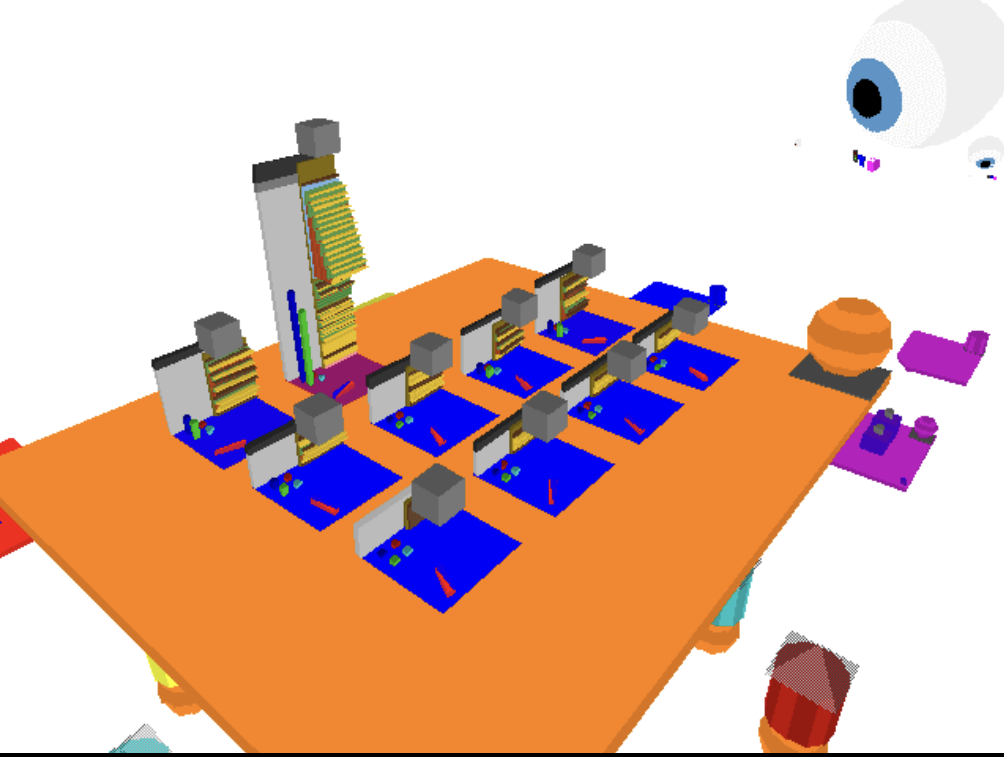
\includegraphics[width=0.5\textwidth]{images/visVRExample.png}
    \caption{Beispiel für eine 3D-Visualisierung von Young und Munro \cite[6]{visSoftwareVR}}
    \label{fig:3DVis}
\end{figure}

Trotzdem können wir auch für unser Ziel der Software-Qualitätsmetrik-Visualisierung Kriterien ableiten, die für eine gute Visualisierung wichtig sind \cite{visSoftwareVR}:
\begin{itemize}
    \item \textbf{Darstellung}: Der wichtigste Aspekt ist die Darstellung der Software. Die Visualisierung sollte die Struktur und den Aufbau der Software verdeutlichen. Die Frage ist also, wie wird die Software dargestellt? 
    \begin{itemize}
        \item Informationsgehalt: Die Visualisierung sollte so viele Informationen wie möglich enthalten.
        \item Niedrige visuelle Komplexität: Als Gegenspieler zum Informationsgehalt steht die visuelle Komplexität. Die Visualisierung sollte so einfach wie möglich gehalten werden, um den Betrachter nicht zu überfordern.
        \item Skalierbarkeit: Die Visualisierung sollte auch bei großen Software-Systemen noch gut lesbar sein. Dies ist besonders wichtig, da wir hier über große Software-Systeme sprechen. Die Autoren von \textit{Visualising Software in virtual reality} \cite{visSoftwareVR} sagen zudem, dass mechanismen Nötig sind, um Komplexität und Informationsgehalt zu steuern und je nach Software-System anpassen zu können.
        \item Stabilität gegenüber Änderungen: Die Visualisierung sollte stabil gegenüber Änderungen in der Software sein. Das bedeutet, dass die Visualisierung sich nur so sehr wie nötig ändert, wenn sich die Software ändert, um eine Versions konsistente Vergleichbarkeit zu ermöglichen und bereits mit der Visualierung vertraute Nutzer nicht zu überfordern.
        \item Gute Visuelle Metaphern: Die Visualisierung sollte gute visuelle Metaphern verwenden, um bereits bekannte Konzepte zu verwenden, um die Software verständlicher zu machen.
    \end{itemize}
    \item \textbf{Abstraktion}: Das Ziel von Visualierung muss sein, unwichtige Details auszublenden und ein verständliches Modell der Software zu erstellen.
    \item \textbf{Navigation}: Da wir häufig über große Software-Systeme sprechen, kann es schnall passeiren dass Nutzer in der Visualisierung verloren gehen. Es muss also möglich sein, sich gut zurecht zu finden und intuitiv zu wissen, wo was ist, um so ein grfühl für die software zu erhalten.
    \item \textbf{Korrelation mit dem Code}: Die Visualisierung sollte eine gute Korrelation mit dem Code haben. Wenn man die Visualierung sieht, soll man diese auch mit dem Code in Verbindung bringen können. Es sollte also möglich sein, die Visualisierung mit dem Code zu verknüpfen und so ein besseres Verständnis für die Software zu bekommen.
    \item \textbf{Automatisierung}: Die Visualisierung sollte automatisiert werden können - ein Punkt der trivialier weise gegeben ist, da wir hier über algorithmen sprechen, die keine manuelle eingabe benötigen.
\end{itemize}

\subsubsection{CodeCity} \label{sec:CodeCity}
Der Cornerstone von 3D Software-Qualitätsvisualisierung ist das Konzept von CodeCity \cite{codeCity1}. Das Paper von Richard Wettel und Michele Lanza verbindet einige Aspekte, die zu diesem Zeitpunkt neu waren. Sie reden zwar nicht konkret von software-qualitäts-visualierung, nutzen aber trotzdem qualitätsmetriken auf Klassenebene, um die richtige Granulariät von Software visualierung zu finden. Herkommliche paper waren oft noch auf niedrigeren ebenen z.b. Marcus Adrian et al. auf Ausdrucks-Ebene \cite{3dsoftwareMarcus}. Zudem nutzen sie, wie von Young und Munro \cite{visSoftwareVR} gefordert, eine gute visuelle Metapher, um die Software darzustellen. Sie nutzen das Konzept einer Stadt, um die Software darzustellen. Dabei wird jede Klasse als Gebäude dargestellt, dabei hat jedes Artefakt (Klassen, Pakete und Ordner) verschiedene Attribute: Die Dimension, die Position, die Farbe, die Farbsättigung und die Transparenz. Ein Beispiel für eine solche Visualisierung ist in Abbildung \ref{fig:codeCity} dargestellt.

\begin{figure}
    \centering
    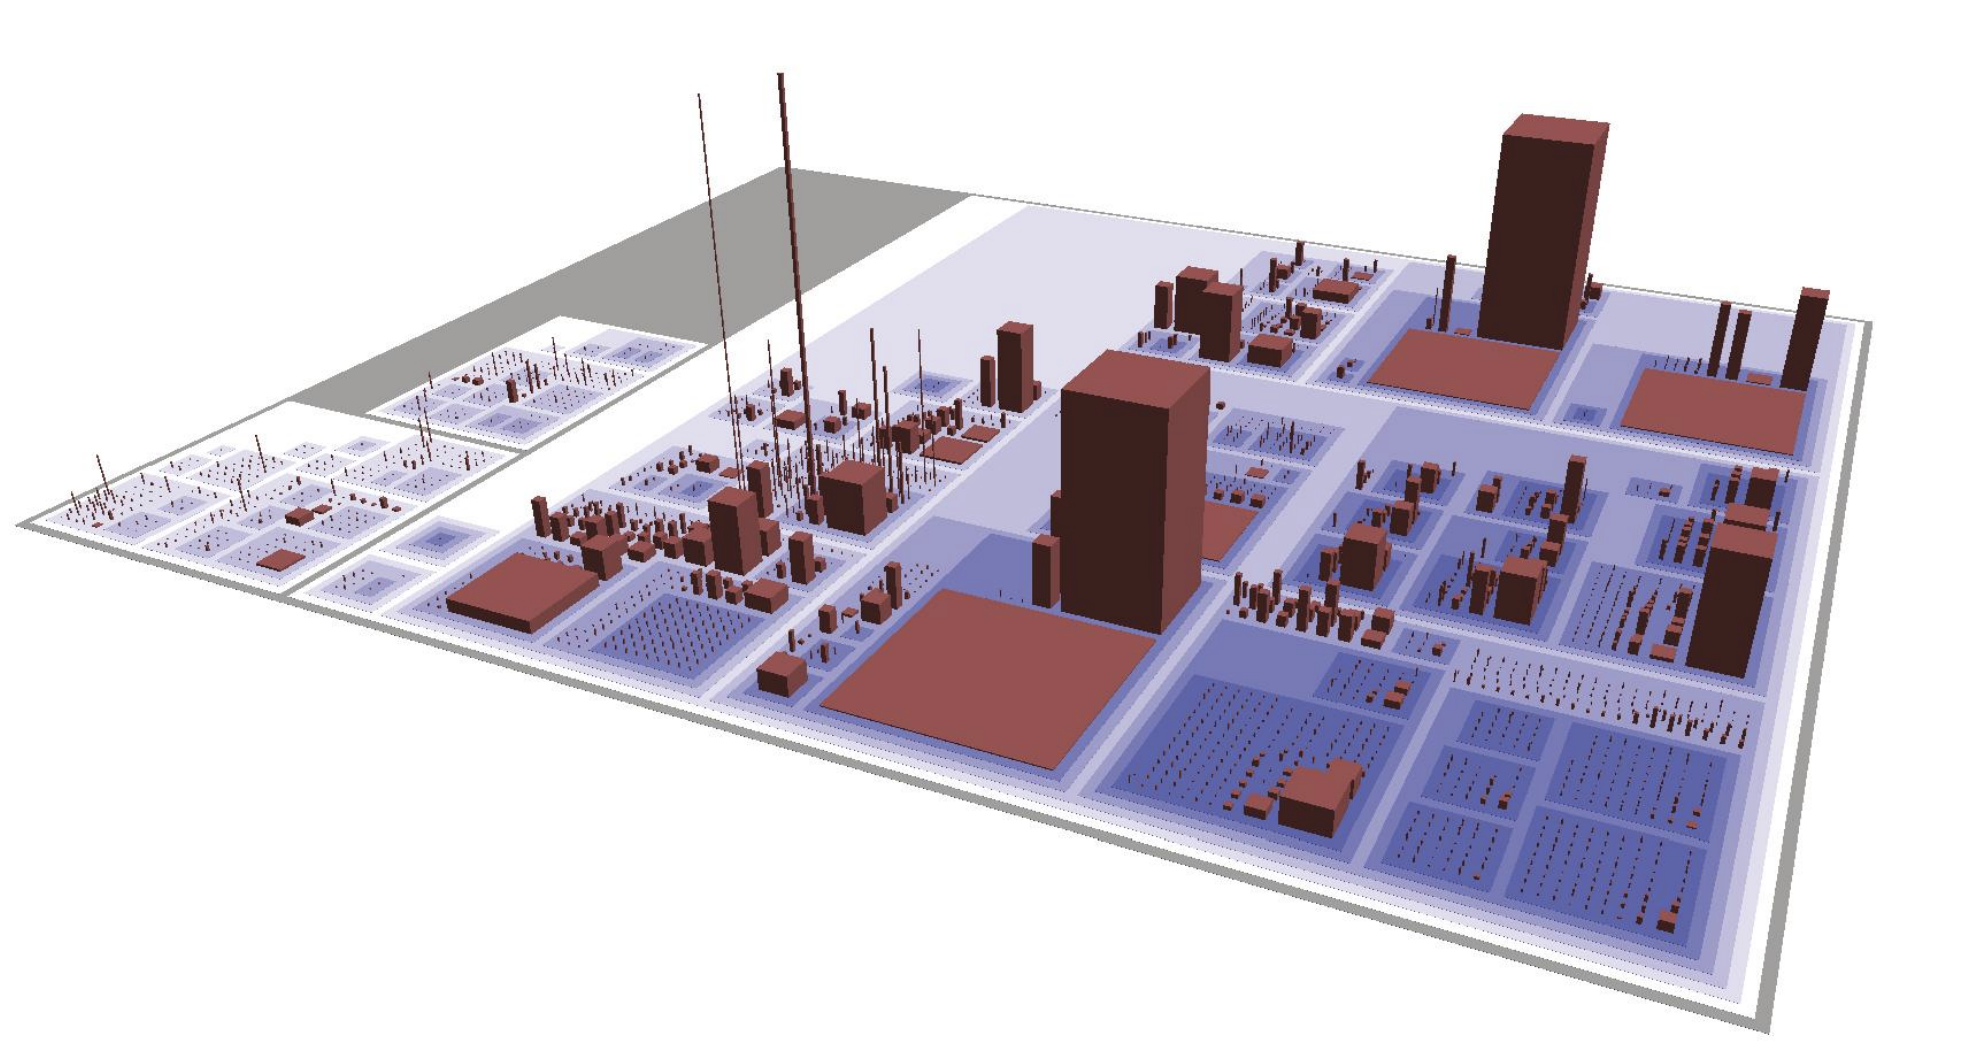
\includegraphics[width=0.5\textwidth]{images/codeCityExample.png}
    \caption{Beispiel für eine original CodeCity-Visualisierung \cite[2]{codeCity1}}
    \label{fig:codeCity}
\end{figure}

Das Layout der Stadt wird lässt sich dabei herunterbrechen auf ein 2D-Layout Problem. Um dieses problem zu lösen, implementieren sie eine abwandlung von Treemap-Algoithmen (Was treemaps sind wird in abschnit \ref{sec:Treemap} erklärt). Auffällig bei Ihrer implementierung ist, dass es viele ungenutzte leere flächen ohne gebäude gibt und gebäude anhand ihrer Größe sortiert plaziert werden (groß weiter unten links, klein weiter oben rechts). Leider ist der algotihmus nicht frei zugänglich, sodass in dieser Arbeit zum vergleich eine eigene Implementierung des Algorithmus verwendet wird, wodurch natürlich auch die Ergebnisse, von der original implementierung abweichen werden (außer wenn anders gekennzeichnet).

\subsection{Treemap-Layouts} \label{sec:Treemap}

Eine Treemap visualisiert einen Baum, indem jedem Knoten ein Rechteck mit der Fläche A zugewiesen wird, proportional zu seinem zugewiesenen Wert (z.B. Datenmenge oder Marktwert). Nicht-Blatt-Knoten werden dabei üblicherweise durch Rahmen (Container-Rectangles) gekennzeichnet, um die Gruppierung der Kinder zu zeigen. \cite{bruls2000squarified} Die Rechtecke aller Blätter füllen die Fläche des Wurzelrechtecks vollständig aus. Mathematisch entspricht die Eingabedatenstruktur einem gewichteten Baum, bei dem jede Blatteinheit eine numerische Größe hat. Die Fläche eines Eltern-Rechtecks entspricht der Summe der Flächen (Werte) seiner Kinder.

Die konkrete Idee hierarchische DAten in form von Treemaps darzustellen wurde erstmals 1991 von Shneiderman und Johnson \cite{johnson1991tree} vorgestellt. Sie stellten fest, dass die Darstellung von hierarchischen Daten in Form von Bäumen in der Regel nicht sehr anschaulich ist. Sie entwickelten eine Methode, um diese Daten in Form von Rechtecken darzustellen, die die Fläche der Knoten proportional zu ihrem Wert darstellen. Diese Methode wurde als \enquote{Treemap} bezeichnet. Als Ziele dieser Visualierung formulierten sie unter anderem diese Aspekte:
\begin{itemize}
    \item \textbf{Effiziente Nutzung des Platzes:} Generell soll es darum gehen möglichst viele Informationen auf einem kleinen Raum darzustellen.
    \item \textbf{Verständlichkeit:} Die Visualisierung soll so gestaltet sein, dass sie für den Betrachter leicht verständlich ist. Es soll möglich sein schnell und mit nur niedrigem kognitiven Aufwand die dargesllten Informationen zu erfassen.
    \item \textbf{Ästethik:} Die Visualisierung soll ansprechend gestaltet sein.
\end{itemize}

Zuvor bestehende Ansätze zur Visualisierung von hierarchischen Daten waren in der Regel nicht sehr anschaulich, besonders, wenn es um große Datenmengen ging. Listen, Baumdiagramme (siehe Abbildung \ref{fig:baumdiagramm}) oder andere Darstellungen (auch bekannt als Node oder Link-Diagramme) sind nicht in der lage alle diese Aspekte zu erfüllen. Bei Einem typischen Baumdiagram zum Beispiel werden teilweise mehr als die Hälfte der Fläche für Hintergrund genutzt \cite[3]{johnson1991tree} außerdem ist es schwer, außer der Struktur der Daten auch die Metriken darzustellen. Sie kritisieren auch die Darstellung von hierarchischen Daten in Form von Venn-Diagrammen (siehe Abbildung \ref{fig:venndiagram}): \enquote{The space required between regions would certainly preclude this Venn diagram representation from serious consideration for larger structures.}\cite[5]{johnson1991tree} Es ist zwar möglich durch die Größe der Kreise eine Metrik darzustellen, es sei aber nicht möglich eine große Anzahl an Knoten sinnvoll darzustellen. 

\begin{figure}[ht]
    \centering
    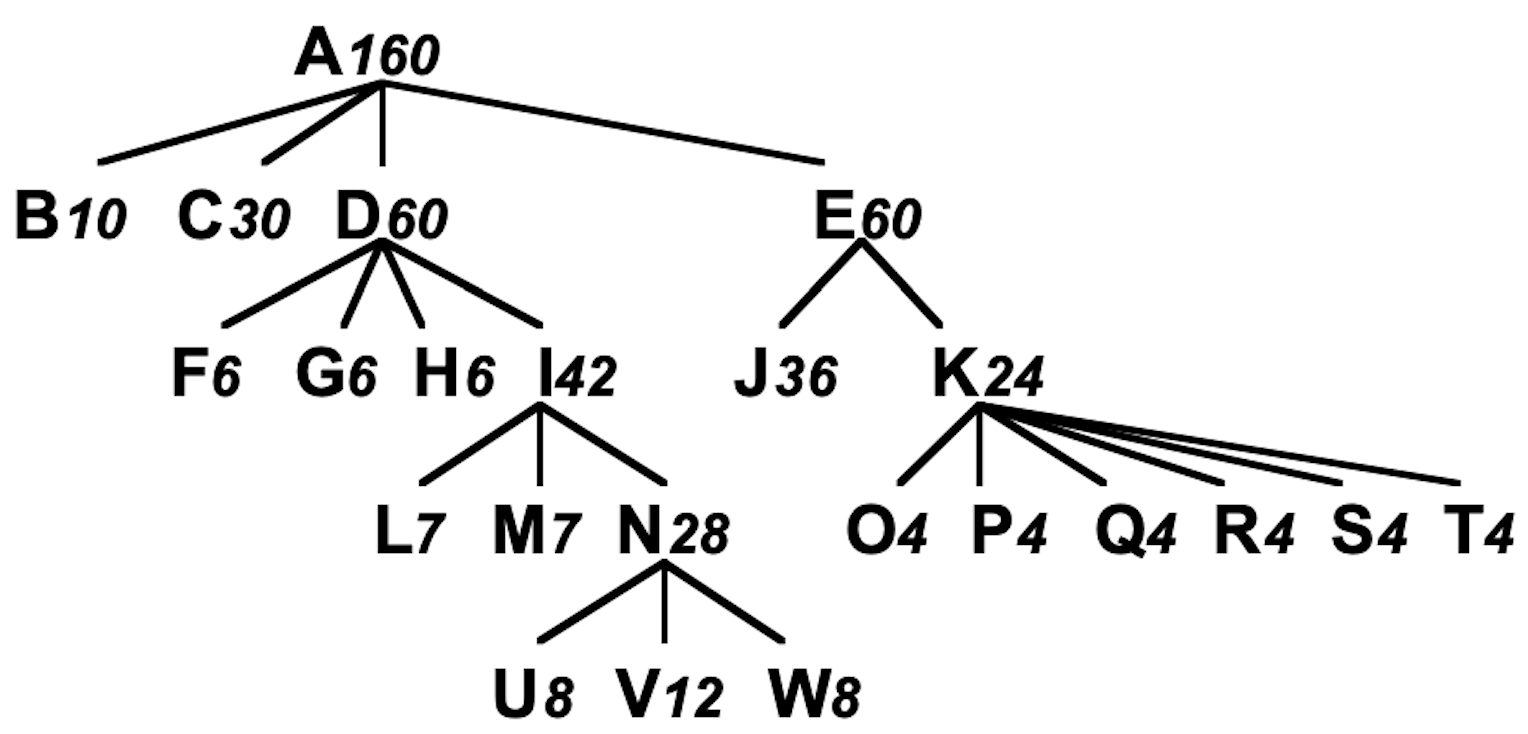
\includegraphics[width=0.5\textwidth]{images/treediagram.png}
    \caption{Beispiel für ein Baumdiagramm}
    \label{fig:baumdiagramm}
\end{figure}

\begin{figure}[ht]
    \centering
    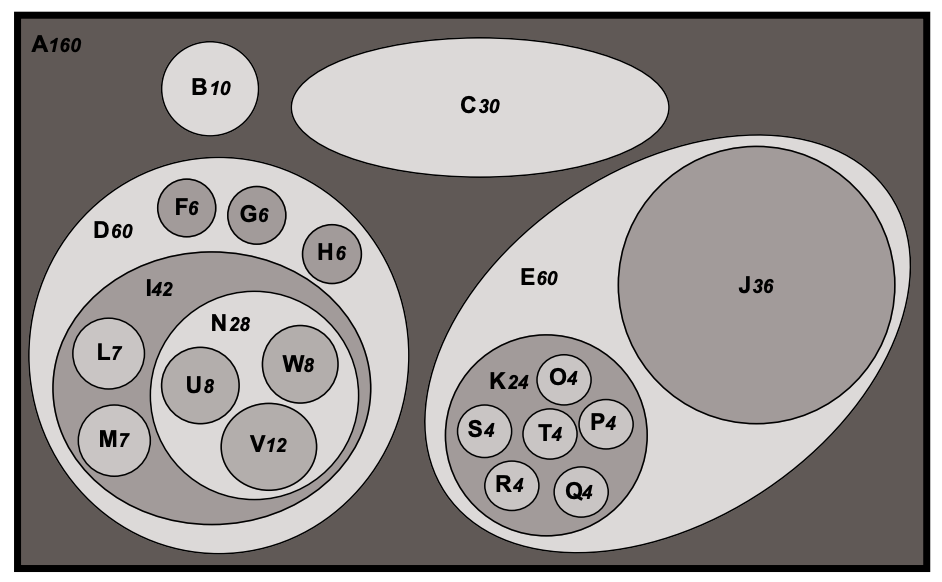
\includegraphics[width=0.5\textwidth]{images/verdiagram.png}
    \caption{Beispiel für ein Venn-Diagramm}
    \label{fig:venndiagram}
\end{figure}

\enquote{Using boxes instead of ovals and a bin-packing algorithm could partially solve this space
problem. But bin-packing is an NP-complete problem and does not preserve order.}\cite[5]{johnson1991tree} Sie stellen fest, dass es theoretisch eine dem Venn Diagramm ähnliche Lösung gibt, die allerdings NP-Hard ist. 

\begin{figure}[ht]
    \centering
    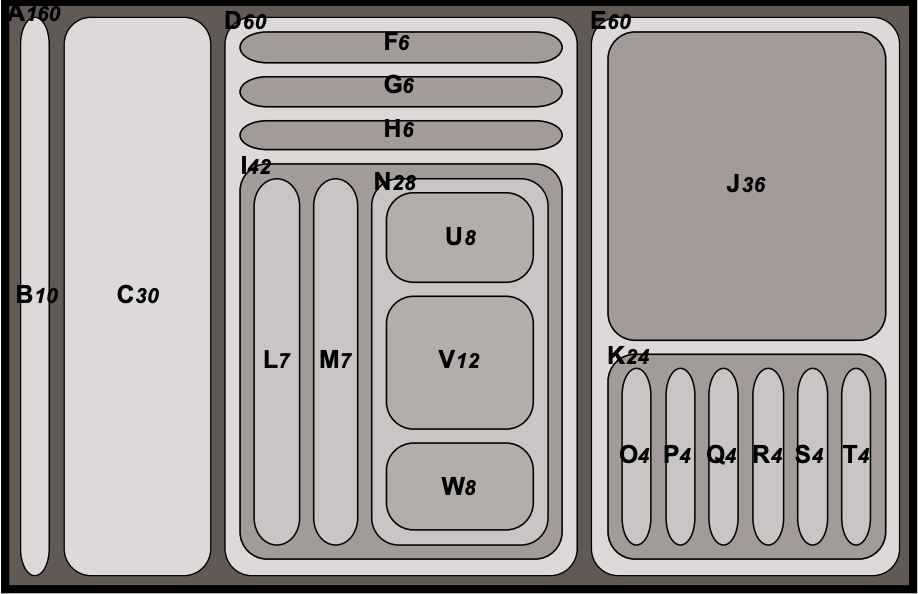
\includegraphics[width=0.5\textwidth]{images/rectVennDiagram.png}
    \caption{Beispiel für ein Boxed Venn-Diagramm}
    \label{fig:rectVennDiagramm}
\end{figure}

Shneiderman und Johnson schlagen zur Lösung dieser Schwierigkeiten ihren Treemap ansatz vor. Sie legen vier Eigenschaften fest, die bei der Erstellung der Treemaps gewährleistet werden:

\begin{itemize}
    \item Wenn ein Knoten 1 ein Vorfahre von Knoten 2 ist, dann ist der Bereich von Knoten 1 vollständig enthalten in dem Bereich von Knoten 2.
    \item Die Bereiche von zwei Knoten schneiden sich, wenn ein Knoten ein Vorfahre des anderen ist.
    \item Knoten belegen eine Fläche, die streng proportional zu ihrem Gewicht ist.
    \item Das Gewicht eines Knotens ist größer oder gleich der Summe der Gewichte seiner Kinder.
\end{itemize}

Sie stellen auch einen Algorithmus vor, der diese Eigenschaften erfüllen soll. Ein von diesem Algorithmus erzeugtes Layout ist in Abbildung \ref{fig:nestedTreemap} dargestellt. 

\begin{figure}[ht]
    \centering
    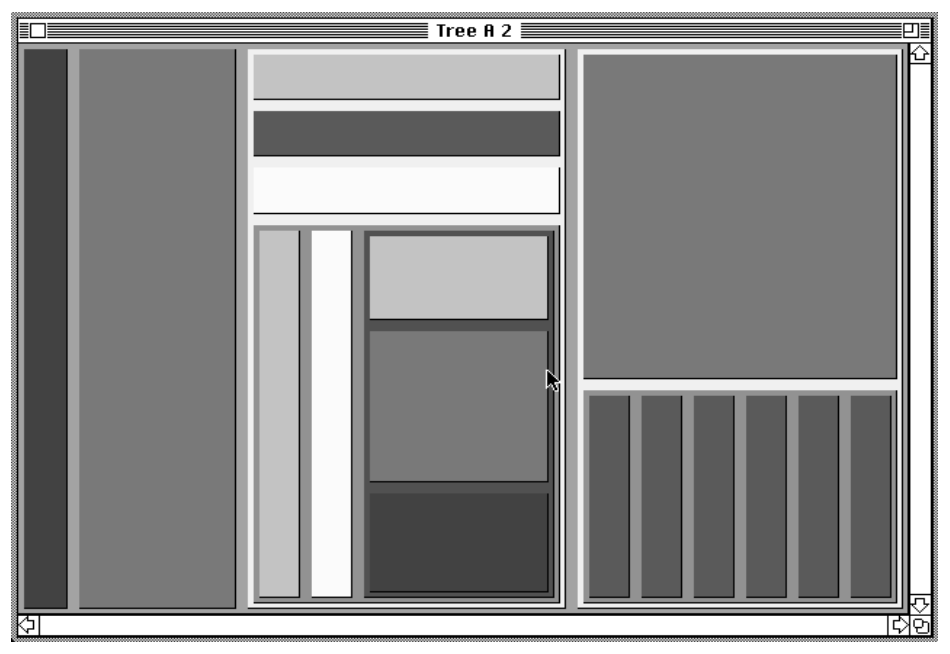
\includegraphics[width=0.5\textwidth]{images/nestedTreemapDiagramm.png}
    \caption{Beispiel für eine Treemap}
    \label{fig:nestedTreemap}
\end{figure}

Der Algorithmus unterteilt den Raum abwechselnd vertikal und horizontal, je nach größe der Knoten. Der Algorithmus arbeitet sich rekursiv von der Wurzel bis zu den Blättern herunter und hat eine Laufzeit von O(n), wobei n die Anzahl der Knoten ist. Im nächsten Abschnitt wird ein ähnlicher Algorithmus im Detail beschrieben, was zum besseren verständis dieser Art von Algorithmen helfen wird.

Obwohl es sich hier um ein renomiertes und viel Zitiertes Paper handelt, machen die Authoren einen entscheidenden Fehler, der in manchen Fällen sogar dazu führen kann, dass Rechtecke komplett verschwinden. Die Authoren betrachten dieses Problem in ihrem Paper leider nicht. 
Der Abstand zwischen den Knoten wird nämlich dadurch erzeugt, dass die Rechtecke diesen Abstand links, recht, oben und unten abgezogen bekommen. Dadurch ist die dargestellte Fläche der Rechtecke nicht mehr proportional zu den Werten, die sie darstellen sollen. Eigenschaft 3 wird also verletzt. Dies ist besonders problematisch, wenn die Rechtecke sehr klein bzw. sehr langgezogen sind. In diesem Fall kann es dazu kommen, dass die Rechtecke so klein werden, dass sie nicht mehr dargestellt werden können. Dies stellt in der Praxis ein riesiges Problem dar, speziell wenn das Problem dieser Arbeit also 3D im kopf bahalten wird. Es kann ja theoretisch vorkommen, dass als Flächenmetrik die lines of code verwendet wird und dort ein file, weil er wenige lines hat sehr klein wird und deswegen aufgrund der margins nicht angezeigt wird. Wenn jetzt aber die metrik für die Höhen berechnung die prozentualle test abdeckung der lines ist und der file nicht getestet ist, dann würde ein potentiell großes problem, was auch eigentlich direkt in auge springen sollte, nicht angezeigt werden. 

Ein weiteres Problem bei diesem Algorithmus ist auch generell, dass unter umständen die Rechtecke sehr langgezogen werden können, was unter Umständen auch Kriterium 3 der Ästethik verletzt. Es gibt viele Ideen dieses Problem anzugehen. Eine Möglichkeit, den Squarify Algorithmus zu verwenden, wird im nöchsten Abschnitt vorgestellt.

Zuletzt noch eine klarstellung im Bezug auf die erweiterung von 2D treemaps um eine Dimension. In der Literatur kommt es hier öfter zu unklarheit. Eigenlicht sind 3D treemaps so ähnlich wie 2D treemaps, nur dass sie anstatt ein rechteck zu unterteilen. Würfel bzw Quader unterteilen, wobei dann nicht die Fläche sondern das Volumen betrachtet wird. In dieser Arbeit geht es aber nicht darum, sondern um sogenannte 2.5D Treemaps, wobei das 2D Treemap layout nach oben extrudiert wird, um eine dritte Dimension zu erhalten. Wenn in dieser ARbeit also von 3D Darstellung die Rede ist, dann ist damit im Kontext von Treemaps eigentlich eine 2.5D Treemap gemeint.

\subsubsection{Squarify-Algorithmus} \label{sec:Squarify}

Der Squarify-Algorithmus ist ein Layout-Algorithmus für Treemaps, der darauf abzielt, die Fläche der Rechtecke so ausgewogen wie möglich zu gestalten. Beduetet, dass die Rechtecke möglichst quadratisch sind. Die ursprüngliche form des algorithmusses wurde im Jahr 2000 von Bruls et al. \cite{bruls2000squarified} vorgestellt. Sie stellten fest: \enquote{another problem of standard treemaps [is] the emergence of thin, elongated rectangles}\cite[1]{bruls2000squarified}. wenn rechtecke nicht mehr so langgezogen sind, Es ist einfacher auf Rechtecke zu zeigen, diese wahrzunehmen, sie zu vergleichen und ihre größe einzuschätzen. 

Der Algorithmus arbeitet rekursiv und teilt die Fläche in Rechtecke auf, wobei er versucht, die Seitenverhältnisse der Rechtecke so nah wie möglich an 1 zu halten. Sie stellen einen rekursiven Ansatz vor, bei dem, wie auch bei den meisten anderen Treemap-Algorithmen, die Rechtecke von oben nach unten (also vom Wurzelknoten bis zu den Blattknoten) aufgeteilt werden.

Im Folgenden wird der Algorithmus beschrieben, da er eine wichtige Grundlage für das Verständnis des Problems darstellt und außerdem eine gute Grundlage zum Verständnis der anderen Algorithmen bietet, da viele Algorithmen ähnliche Ideen verwenden.

Der Algorithmus wird anhand eines Beispiels aus dem originalen Squarify-Paper \cite[5]{bruls2000squarified} erläutert. Wir werden den Algorithmus jedoch anders erklären als im Paper, da wir uns näher an der Implementierung orientieren, wie sie in der bekannten d3-Bibliothek \cite{d3_treemap_code} umgesetzt ist.
Es sollen Rechtecke mit den Größen 6, 6, 4, 3, 2, 2, 1 in ein 6 mal 4 Rechteck einsortiert werden.

Der algorithmus arbeitet immer in Reihen, die er versucht zu füllen und dabei die Rechtecke möglichst quadratisch zu halten. Das erste Rechteck ist breiter als lang. (In dieser Arbeit werden wir, anders als in den herkömmlichen papern zu layout algorithmen, das Wort breit als x koordinate und das wort lang als y koordinate nutzen - das hat den hintergrund, dass das wort hoch im drei dimensionalen meist für die z komponent genutzt wird und es sonst zu verwirrungen kommen könnte)
Da das Rechteck in das wir einfügen breiter als lang ist, werden wir eine imaginäre horizontale Reihe so lange mit Rechtecken befüllen, bis ein Threshold erreicht ist. Das erste Rechteck mit größe 6 fügen wir also in Schritt 1 in diese Reihe ein. Das Seitenverhältnis dieses Rechtecks beträgt 8 zu 3 (das Rechteck ist 1.5 Einheiten breit und 4 Einheiten lang). Das zweite Rechteck mit größe 6 fügen wir in Schritt 2 in diese horizontale Reihe ein, dabei wird die Reihe entsprechend breiter. Das Seitenverhältnis des jetzt eingefügten Rechecks beträgt 3 zu 2 (das Rechteck ist 3 Einheiten breit und 2 Einheiten lang). Jetzt kommt das nächste Rechteck mit größe 4. Dieses Rechteck ist hat ein Seitenverhältnis von 4 zu 1 (das Rechteck ist 4 Einheiten breit und 1 Einheit lang). Das hinzufügen dieses Rechtecks führt nun aber dazu, dass das schlechteste Seitenverhältnis der Reihe von 3 zu 2 auf 4 zu 1 ansteigt. Deshalb wird diese Reihe als abgeschlossen angesehen und die nächste Reihe wird begonnen - Schritt 4. 

Dieser Schritt des suchens des schlechtesten Seitenverhältnisses lässt sich von der rechenkomplexität her gut optimieren, sodass der Ratio berechnet werden kann, ohne dass die Reihe wirklich mit Rechtecken gefüllt werden muss. 
Anstatt für jeder Rechteck max(w/l, l/w) zu berechnen, ziehen wir folgende vereinfachung heran.

\begin{align}
    \frac{w_i}{l_i} 
    &= \frac{w_i \cdot l_i \cdot w^2}{l_i \cdot l_i \cdot w^2} \\
    &= \frac{w_i \cdot l_i \cdot w^2}{l_i^2 \cdot \left(\sum_{j=0}^{n} w_j\right)^2} \\
    &= \frac{w_i \cdot l_i \cdot w^2}{\left(l_i \cdot \sum_{j=0}^{n} w_j\right)^2} \\
    &= \frac{w_i \cdot l_i \cdot w^2}{\left(\sum_{j=0}^{n} l_i \cdot w_j\right)^2} \\
    &= \frac{w_i \cdot l_i \cdot w^2}{\left(\sum_{j=0}^{n} l_j \cdot w_j\right)^2}
    \quad\text{da } \forall i, j \in \{0, \dots, n\}, l_i = l_j \\
    &= \frac{V_i \cdot w^2}{sV^2}
\end{align}
Analog dazu gilt das gleich auch für $ \frac{l_i}{w_i} = \frac{sV^2}{V_i \cdot w^2} $. Da wir nur an dem maximalen Wert beider Ausdrücke interessiert sind und die Länge ($l_i$) aller Rechtecke in der Reihe gleich ist, reicht es den Wert für das größte und das kleinste Rechteck zu berechnen und davon den maximalen Wert zu nehmen.

$w$ ist für den gesamten Zeitraum des füllens einer Reihe konstant und muss daher nur einmal berechnet werden. $sV$ wird mit jedem Rechteck aktualisiert. 

Das Ziel ist es das Verhältnis der Seitenlängen gleich zu halten. Im ursprünglichen Paper von Bruls et al. \cite{bruls2000squarified} wird darauf noch nicht so eingegangen, aber viele implementierungen z.b. die von d3.js \cite{d3_treemap_code} ermöglichen es, das Verhältnis nicht nur an den Wert 1 anzunähern, sondern auch an andere Werte, zum Beispiel den goldenen Schnitt \cite{goldenRatio}. 

\begin{figure}[h]
    \centering
    
\includegraphics[width=0.5\textwidth]{images/oneSquarify.png}
    \caption{Beispiel für ein Squarify-Layout mit Annäherung an quadratische Rechtecke (Durchschnittliches Seitenverhältnis 1.42)}
    \label{fig:squarifyRatio1}
\end{figure}

\begin{figure}[h]
    \centering
    
\includegraphics[width=0.5\textwidth]{images/fiveSquarify.png}
    \caption{Beispiel für ein Squarify-Layout mit Annäherung an den Wert 5 (Durchschnittliches Seitenverhältnis 2.79)}
    \label{fig:squarifyRatio5}
\end{figure}

%wie wirkt sich die reihenfolge auf das layout aus?
%was ist mit kd-bäumen
\section{Problemstellung} \label{sec:Problemstellung}
Die fundamentale und schwerste Frage, bei den Stadt-Analogien ist, wie das Layout der Stadt aussehen soll.

\subsection{Das Treemap Problem} \label{sec:TreemapProblem}
In Abschnnit \ref{sec:Treemap} wurde aufgezeigt, dass bereits der initiale Algorithmus von Johnson und Shneiderman \cite{johnson1991tree} ein fundamentales Problem aufweist, wenn Treemaps mit Abständen zwischen Knoten dargestellt werden sollen. 
\begin{itemize}
    \item Da der Abstand von der Fläche der Knoten abgezogen wird, ist die dargestellte Fläche nicht mehr proportional zum Wert des Knotens.
    \item Durch das Abziehen der Abstände kann es passieren, dass Knoten verschwinden, wenn entweder die Länge oder die Breite der Knoten kleiner oder gleich dem Abstand ist.
\end{itemize}

Es ist nicht trivial dieses Problem zu lösen, da es die grundlegende Annahme der Treemap Algorithmen verletzt, dass die Fläche aller Knoten bekannt ist, bevor die Knoten plaziert werden. 
Bevor die Knoten plaziert werden, ist nicht klar, wie die Fläche der Knoten aussieht, das heißt, es ist auch nicht klar, wie viel Platz für die Abstände zwischen den Knoten benötigt wird. Dies wird klar wenn man sich die Abbildung \ref{fig:marginAreaDifference} anschaut. Dort sieht man, dass die Fläche, die für Knoten in ihren Eltern benötigt wird, größer ist als die Fläche, die für die Knoten selbst benötigt wird und diese benötigte Fläche stark vom Layout der Knoten selbst abhängt. Somit ist auch unklar, wie groß die Fläche aller elternknoten sind. 

\begin{figure}
    \centering
    
\includegraphics[width=0.8\textwidth]{images/marginArea.png}
    \caption{Abbildung eines zweier Rechecke mit der Fläche 16 in dunkel grau und in hellgrau der Abstand von 1 um die Flächen herum. Das Linke Rechteck (4x4) mit Abstand nimmt eine Fläche von 25 (5x5) ein. Das rechte Rechteck (2x8) mit Abstand nimmt eine Fläche von 40 (4x10) ein.}
    \label{fig:marginAreaDifference}
\end{figure}

Das Problem ist jetzt aber, dass wenn die Fläche der Knoten nicht bekannt ist auch das Layout der Knoten nicht berechnet werden kann, da die Fläche der Knoten für das Layout benötigt wird. Hier ergibt sich also ein Zirkelschluss: Die Fläche ist nicht klar, ohne das Layout und das Layout kann nicht berechnet werden, ohne die Fläche zu kennen.

\section{Ziel} \label{sec:Ziel}

Laut Marcus Adrian et al.  gibt es 5 Dimensionen die man beachten muss, wenn es um software visualierung geht: 
\begin{quote}    
    • Tasks - why is the visualization needed?
    • Audience - who will use the visualization?
    • Target - what is the data source to represent?
    • Representation - how to represent it?
    • Medium - where to represent the visualization? \cite[2]{3dsoftwareMarcus}
\end{quote}

Wir beantworten diese Fragen, um das Ziel dieser Arbeit zu begründen.
\textbf{Warum ist die Visualisierung von Codequalitätsmetriken wichtig?}
Die Visualisierung von Codequalitätsmetriken ist wichtig, um die Qualität von Softwareprojekten zu bewerten und zu verstehen, aber auch um einen schnellen Überblick über die Codebasis zu geben und einen Einstieg in vertiefende Codeanalysen zu ermöglichen. Eine effektive Visualisierung kann helfen, schnell Hotspots im Code zu identifizieren, die möglicherweise verbessert werden müssen, und somit die Wartbarkeit und Qualität des Codes zu erhöhen. Außerdem soll die Visualisierung ermöglichen verschiedene Metriken in verbindung zu setzen, um so eine höhere Aussagekraft über den Code, den die einzelne betrachtung jeder Metrik nicht bieten kann.
Der wichtigste Punkt ist, das subjektive \textit{Greifbar} machend der CodeQualität.

\textbf{Wer wird die Visualisierung nutzen?}
Die Visualisierung ist vorallem an Personen gerichtet, die sich nicht mit der Codebasis auskennen. Das können Entscheidungsträger sein, die keine ahung von software entwicklung haben, das können aber auch entwickler sein, die sich neu in ein Projekt einarbeiten müssen, um die qualität einer software zu erhöhen.

\textbf{Was ist die Datenquelle?}
Die Datenquelle sind hierarschiche Codequalitätsmetriken, die aus dem Quellcode eines Softwareprojekts extrahiert werden. 
Dabei wird jeder Knoten in dieser Hierarchie als "Node" bezeichnet.
Jede Node hat folgendes Schema:
```json
"node": {
    "name": string,
    "children": List[Node] | "value": number,
}
```


\textbf{Wo soll die Visualisierung dargestellt werden?}
Die Visualisierung soll digital auf herkömmlichen Bildschirmen dargestellt werden. Speziell wird in dieser Arbeit beispielhaft eine darstellung in einem Webbrowser angestrebt und die Algorithmen in Typescript implementiert. Natürlich können aber alle Ergebnisse auch in anderen Programmiersprachen und Umgebungen umgesetzt werden.


\textbf{Wie soll die Visualisierung dargestellt werden?}
Im GRunde soll eine Visualierung in Anlehnung an den in Abschnitt \ref{sec:CodeCity} beschriebenen Stadt-Metapher ansatz verfolgt werden. - Speziell soll es in dieser Arbeit um das Layout der Knoten gehen, aber im hinterkopf soll die stadtmetapher bleiben und immer als grundlage für die bewrtung des 2d layouts dienen. 
Wie in der CodeCity arbeit beschrieben, soll es möglich sein Metriken in form von Fläche, Höhe und farbe (ob jetzt nur farbe oder durchsichtigkeit wie bei dem codecity paper oder sogar textur von knoten - wird hier ignoriert). Das heißt also, dass das 2D layout in gewisser weise eingeschtränkt wird, zB. wenn Farbe als visulaisrung von struktur verwendet werden soll oder wie in \cite{bruls2000squarified} schattierung.

Speziell soll die Visualisierung am Ende optimiert auf folgende Aspekte sein, die sich aus den im Abschnitt \ref{sec:Grundlagen} beschriebenen Grundlegenden Aspekten von Softwarevisualierung, leicht angepasst and das Problem dieser Arbeit, ableiten lassen: 

\begin{itemize}
    \item \textbf{Informationsgehalt und Effiziente Nutzung des Platzes:} Die Visualisierung sollte so viele Informationen wie möglich auf so wenig Platz wie möglich darstellen.
    \item \textbf{Niedrige visuelle Komplexität und Verständlichkeit:} Als Gegenspieler zum Informationsgehalt steht die visuelle Komplexität. Die Visualisierung sollte so einfach und verständlich wie möglich gehalten werden, um den Betrachter nicht zu überfordern.
    \item \textbf{Skalierbarkeit:} Die Visualisierung sollte auch bei großen Software-Systemen noch gut lesbar sein. Dies ist besonders wichtig, da wir hier über große Software-Systeme sprechen.
    \item \textbf{Korrelation mit dem Code:} Die Visualisierung sollte eine gute Korrelation mit dem Code haben. Wenn man die Visualierung sieht, soll man diese auch mit dem Code in Verbindung bringen können. Es sollte also möglich sein, die Visualisierung mit dem Code zu verknüpfen und so ein besseres Verständnis für die Software zu bekommen.
    \item \textbf{Zweitrangig ist Stabilität gegenüber Änderungen:} Die Visualisierung sollte stabil gegenüber Änderungen in der Software sein, damit der Qualitätszustand der Software einfacher über die Zeit verfolgt werden kann.
\end{itemize}

\subsection{Kriterien} \label{sec:ZielKriterien}
Um disese fünf Aspekte zu erreichen, definieren wir sechs Kriterien für das 2D layout, die diese Aspekte messbar machen. Diese Kriterien sollen helfen, die Qualität der Visualisierung zu bewerten und zu vergleichen. Die Kriterien sind:

\begin{itemize}
    \item \textbf{Abstände:} Abstände zwischen den Knoten verbessern die Übersichtlichkeit und die visuelle Komplexität.
    \item \textbf{Platznutzung:} Es sollte so wenig Fläche wir möglich ohne Informationsgehalt bleiben. Als gegenbeispiel kann man die Order-Knoten sehen, wie sie in der CodeCity Arbeit beschrieben wurden, bei denen die Fläche der Knoten nicht proportional zur Anzahl der Zeilen im Code ist, wodurch die Fläche an sich keinen Informationsgehalt mehr hat und außerdem viel leere Fläche entsteht.
    \item \textbf{Knoten sichtbarkeit:} Es sollte keine Knoten geben, die aufgrund von Abständen oder anderen Gründen nicht sichtbar sind. Dieses Ziel spielt speziell auf das in abschnitt \ref{sec:Treemap} beschriebene Problem ab.
    \item \textbf{Zeitaufwand:} Die Generierung des Layouts sollte in einem angemessenen Zeitrahmen erfolgen, um eine schnelle Visualisierung zu ermöglichen. Dies verbessert die Skalierbarkeit und generelle Nutzbarkeit der Visualisierung.
    \item \textbf{Seitenverhältnis:} Um die visuelle Komplexität zu reduzieren und die Verständlichkeit zu erhöhen, sollte das Seitenverhältnis der Knoten möglichst nahe bei 1:1 liegen. Dies verbessert die Lesbarkeit der Knoten und macht es einfacher, die Informationen zu erfassen.
    \item \textbf{Flächengröße:} Um die Korrelation mit dem Code zu gewährleisten, sollte die Fläche der Knoten proportional zum Metrikwert sein.
    \item \textbf{Stabilität:} Die Knoten sollten bei Änderungen die Position und Größe beibehalten, um eine stabile Visualisierung zu gewährleisten. 
\end{itemize}

In dieser Arbeit sollen space filling approaches anaylsiert werden und speziell darauf untersucht werden, wie sie sich eignenen für die definierten anforderungen. Wie gut wird was erfüllt? Wann sollte man was anwenden? Kann eine gute kombination aus verschiedenen Ansätzen gefunden werden?
Bisher wurden im Grundlagenteil vorallem die splitting algorhtmen vorgestellt, aber es gibt natürlich auch andere Ansätze, die verfolgt werden können, um Treemap Layouts zu generieren. Zum beispiel gibt es bin packing oder optimierungs algorithmen. In dieser Arbeit sollen auch diese Ansätze betrachtet werden, um zu sehen, ob sie für die Visualisierung von Codequalitätsmetriken in einer space filling layout approach geeignet sind.

Dies soll getestet werden auf basis von verschiedenen öffentlichen Repositories, die von kleinen bis großen Codebasen reichen. Als Metrik für die Fläche soll der Einfachehit halber die Anzahl der Zeilen verwendet werden.


\chapter{Hauptteil} \label{chapter:Hauptteil}
\section{Erweiterung des Squarify Algorithmus} \label{sec:VerbesserungSquarify}
In diesem Abschnitt wird der Squarify Algorithmus \cite{bruls2000squarified}, wie er in Abschnitt \ref{sec:Squarify} beschrieben wurde, auf verschiedene Weisen erweitert und angepasst, um das Layoutproblem, wie es in Abschnitt \ref{sec:TreemapProblem} beschrieben wurde, anzugehen. 

\subsection{Approximative Fläche} \label{sec:ApproxFläche}
Die Grundlegende Idee dieser Erweiterung ist es, die Fläche der Knoten plus die Benötigte Fläche für die Abstände vor berechnung des Layouts zu approximieren.

Dafür brauche ich erstmal einen guten Algorithmus der das Layout gut macht, dann kann ich mit KI die Fläche lernen. Ist die frage ob das wirklich so gut funktionieren kann.

Problem man kann sich sehr gut beispiele konstuieren, bei denen das nicth funktionieren wird. Man kann das natürlich mit skalierung wieder lösen, aber das ist natürlich nicht optimal.

\subsection{Zweifache Berechnung} \label{sec:ZweifachBerechnung}
Die Grundlegende Idee dieser Erweiterung ist es, dass sich die Fläche der Knoten mit Abstand durch das Layout und die Fläche der Knoten ohne Abstand approximieren lässt. Die Idee ist es also einen ersten Durchlauf zu machen, bei dem das Layout ohne Abstand berechnet wird. Dann werden die Größen der Knoten entsprechend dem Layout angepasst, sodass die Größe der Knoten nun auch den Abstand berücksichtigt. Anschließend wird ein zweiter Durchlauf mit diesen angepassten Größen durchgeführt, um das finale Layout zu berechnen.

Bevor wir uns die Details und Ergebnisse dieser Erweiterung anschauen, wollen wir vorweg nehmen, dass diese Erweitung natürlich nicht optimal funktionieren kann und das auch klar ist, da sich die die Änderung der Größe der Knoten natürlich auch das Layout im Zeweiten Durchlauf ändern wird, wodurch die Größen der Knoten wieder nicht korrekt sind. Was ja überhaupt erst das Grundlegende Problem ist (siehe Abshnictt \ref{sec:Problemstellung}). Allerdings ist es ein erster Schritt sich dem Problem zu nähern und zu schauen, ob es sich lohnt in diese Richtung weiter zu forschen.

Der Grundlegende Algorithmus bleibt also (fast) gleich, nur dass zwischen dem ersten und dem zweiten Durchlauf ein zusätzlicher Schritt \textit{Größenanpassung} eingefügt wird. Die Einzige änderung die vorgenommen werden muss ist, dass Knoten nur mit dem definierten Abstand zwischen dem Elternknoten platziert werden können und generell die Fläche des Elternknotens um den Abstand verkleinert wird.
Außerdem ist es nötig nach dem zweiten Durchlauf die Knoten, deren größenwert ja nun den abstand beinhalten, zu verkleinern, um auch den abstand zwischen den Geschwistern herzustellen. Es ist zu erkennen, dass dadurch der Abstand sowohl zwischen Geschwistern als auch zu den Elternknoten den doppelten wert des definierten Abstands hat, dieses Problem ignorieren wir hier, da man es trivialierweise lösen könnte, indem man immer nur die hälfte des Abstands zwischen Geschwistern und Elternknoten abzieht, was wir hier der einfachheit halber nicht tun. -- ODER VIELLEICHT HIER IN DER THESIS DOCH? DANN KÖNNTE ICH MIR DIESEN ABSCHNITT SPAREN, AUCH WENN ES IN DER IMPLEMENTIERUNG AM ENDE ANDERS IST

Wir stellen verschiedene Ansätze vor, was sowohl die Größenanpassung als auch die Anpassung der Knoten nach dem zweiten Durchlauf angeht.
Die Algorithmen funktionieren allerdings alle nach ähnlichem Prinzip: Es wird zunächst für jeden Knoten die Fläche die der Abstand in diesem Layout benötigen würde addiert, indem die Fläche aus der neuen Länge (alte Länge + 2 mal den Abstand) und der neuen Breite (alte Breite + 2 mal den Abstand) berechnet wird. Zusätzlich wird für Elternknoten die Flächenvergrößerung aller Kindernkoten addiert. An dieser Stelle ist allerdings nicht klar, wie sich die Flächenvergrößerung der Kinderknoten auf die Fläche der Elternknoten auswirkt, da diese Änderung selbst von der Anordnung der Kinderknoten abhängt. Wir testen verschiedene Ansätze, um die Flächenänderung der Elternknoten in Abhängikeit zu der Flächenänderung der Kinderknoten zu approximieren.

Nach dem zweiten Durchlauf wird nun die Fläche der Knoten so reduziert, dass sowohl der Abstand zwischen Geschwistern als auch der Abstand zu den Elternknoten den gewünschten Wert hat. Dies ist straight forward und wird hier nicht weiter erläutert. Anzumerken ist aber das dieser Schritt speziell abhängt von der Art der Größenanpassung, die im ersten Schritt durchgeführt wurde.

\subsubsection{Einfache Größenanpassung}
Dies ist die einfachste naive Version der Größenanpassung, der Algorithmus zeigt aber gut die zuvor beschriebenen Probleme auf. Die Fläche der Knoten wird um den Abstand in beiden Richtungen vergrößert. Zusätzlich wird die Fläche der Elternknoten um die Fläche der Kinderknoten vergrößert. 

\begin{algorithm}[H]
\caption{Einfache Größenanpassung}
\label{alg:EinfacheGrößenanpassung}
\begin{algorithmic}[1]
\Function{increaseValuesSimple}{node: SquarifyNode, margin: number}
    \State childrenValueIncrease $\gets$ 0
    \If{node.children}
        \For{child in node.children}
            \State childrenValueIncrease += increaseValuesSimple(child, margin)
        \EndFor
    \EndIf
    \State valueIncrease $\gets$ width * margin * 2 + length * margin * 2 + margin * margin * 4 + childrenValueIncrease
    \State node.value += valueIncrease
    \State \Return valueIncrease
\EndFunction
\end{algorithmic}
\end{algorithm}

Das Problem des Algorithmuses ist am besten an einem Beispiel zu verdeutlichen. Wir visualieren den ZWITEN AnHANG - auch wieder eine händisch erstellte Map, um das Problem zu verdeutlichen. In Abbildung \ref{fig:zeroMarginSquarifyArtifialTwo} ist das Layout mit einem Abstand von 0 zu sehen. 

\begin{figure}
    \centering
    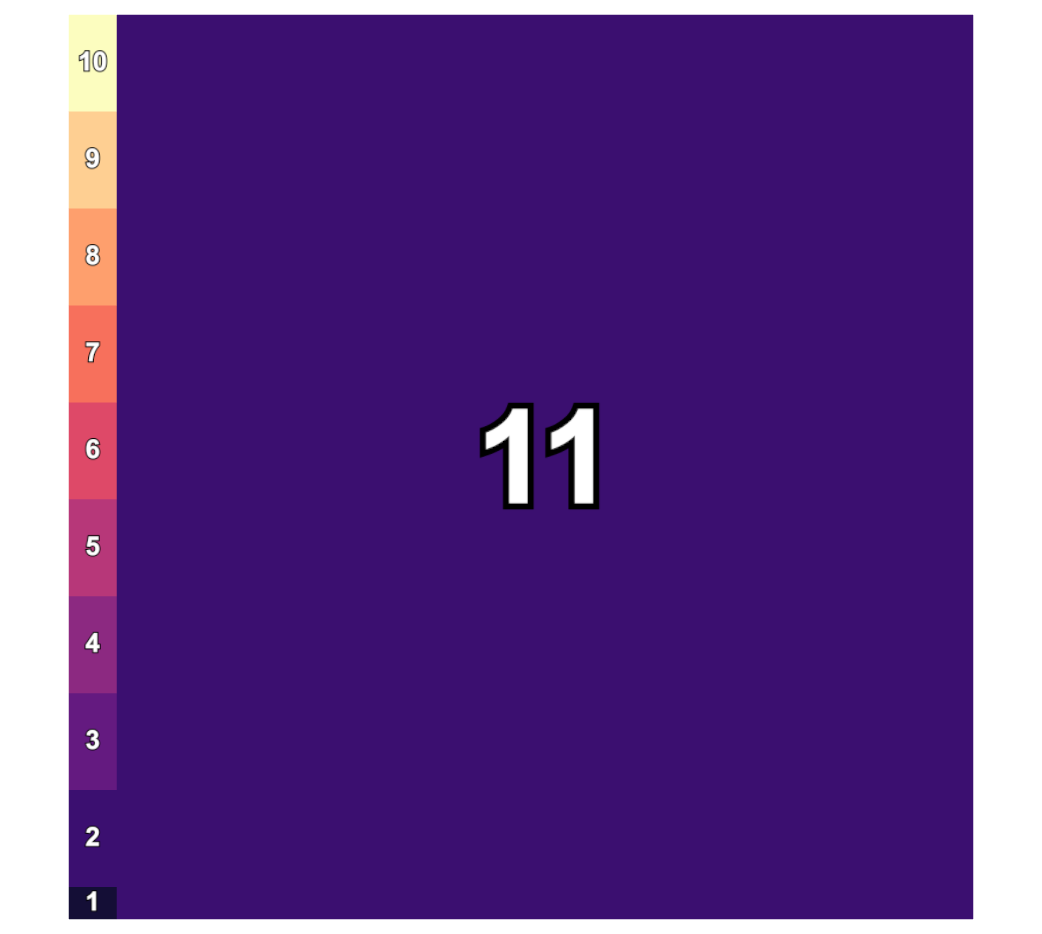
\includegraphics[width=0.8\textwidth]{images/zeroMarginSquarifyArtifialTwo.png}
    \caption{Treemap Layout generiert mit dem Squarify Algorithmus nach Abschnitt \ref{sec:Squarify} mit einem Abstand von 0 und der einfachen Größenanpassung auf der händisch erstellen map (siehe Anhang).}
    \label{fig:zeroMarginSquarifyArtifialTwo}
\end{figure}

In Abbildung \ref{fig:simpleIncreaseMarginOne} ist das Layout mit einem Abstand von 1 zu sehen. Es ist zu erkennen, dass die Knoten auf der linken Seite des Layouts sich außerhalb ihrer Elternknoten erstrecken. Warum passiert das? Knoten 10 ist im zweiten Layout-Schritt deutlich schmaler als im ersten Layout-Schritt. Dadurch wird die Fläche die durch den Abstand eingenommen wird größer als angenommen, weshalb die Fläche des Knotens nach abzug des Abstands im letzen Schritt kleiner ist, als gewünscht. Dementsprechend ist auch die Fläche der Knoten unten links größer als gewünscht, da das Layout der Knoten im zweiten Layout-Schritt quadratischer wird. Knoten 5, der Knoten, der am Quadratischsten ist, wird also am größten erscheinen. Obwohl beide den selben wert haben ist Knoten 5 ca. 1,2 mal größer als Knoten 10) In diesem Beispiel erscheint der unterschied kaum merklich, aber es gibt ihn trotzdem und in anderen fällen kann dieser Unterschied merklich werden.
Viel signifikanter ist aber der Effekt, dass Elternknoten ebenfalls immer schmaler werden, wodurch die fläche, die der innerere abstand einnimm, ebenfalls größer wird und dass sogar immer mehr von ebene zu ebene, wenn man runter geht. Dadurch wird die Fläche für die Kindknoten immer kleiner, was dazu führt, dass Knoten teilweise über ihre Elternknoten hinauswachsen.

\begin{figure}
    \centering
    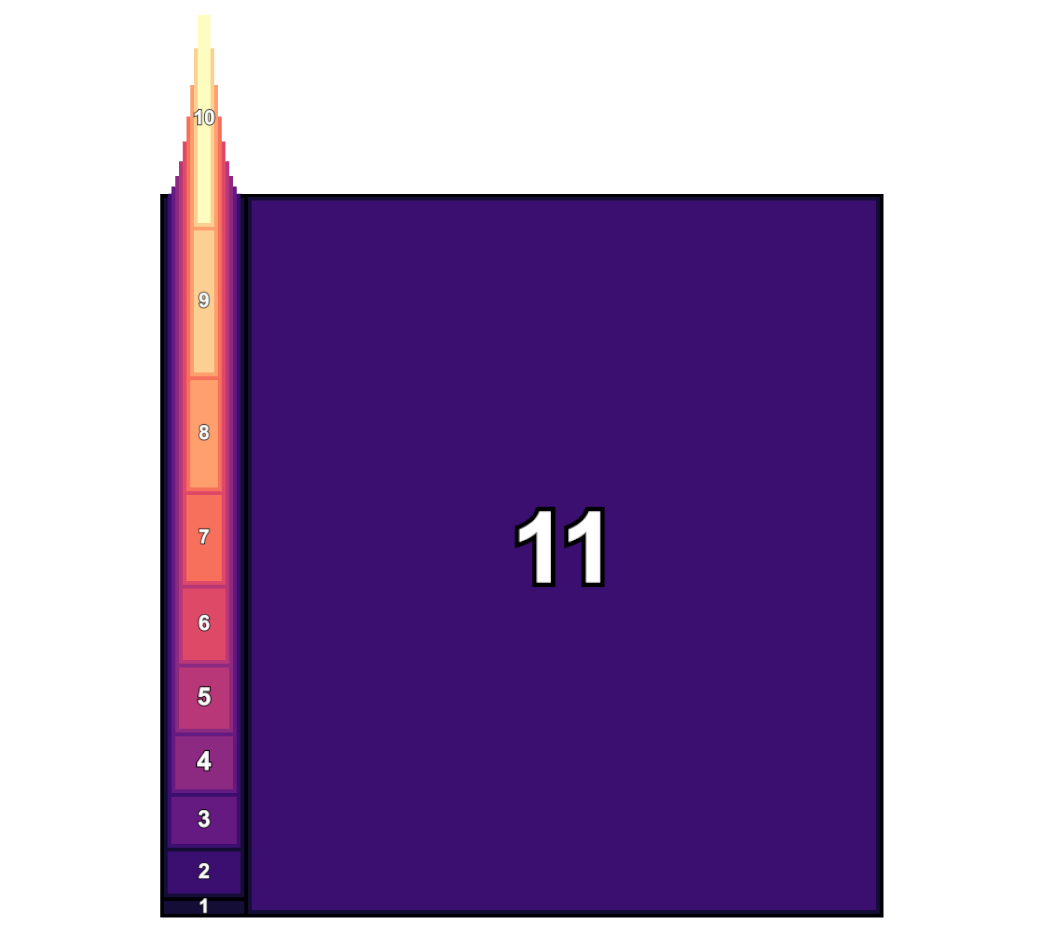
\includegraphics[width=0.8\textwidth]{images/simpleIncreaseMarginOne.png}
    \caption{Treemap Layout generiert mit dem Squarify Algorithmus nach Abschnitt \ref{sec:Squarify} mit einem Abstand von 1 und der einfachen Größenanpassung auf der händisch erstellen map (siehe Anhang).}
    \label{fig:simpleIncreaseMarginOne}
\end{figure}

Dieser Effekt kann einfach behoben werden, wie wir in Abschnitt \ref{sec:ScalingKnoten} sehen werden.

\subsubsection{Relative Größenanpassung}
Bei der berechnung zuvor wurde einfach der margin fläche eines Elternknotens berechnet, auf basis der alten Fläche, ohne die Flächenädnerung durch die Kinderknoten zu berücksichtigen. dadurch wird die resultierende Fläche der Elternknoten zu klein sein, da die Fläche der Kinderknoten nicht berücksichtigt wird.
Die Idee bei dieser Erweiterung ist es die Änderung der Kinder schon vor dem Hinzufügen der Abstandsfläche zu berücksichtigen. Dafür muss die relative Flächenänderung durch die Kindknoten berechnet werden. und damit dann die Seitenlängen anpassen und dann die margins hinzufügen, um die neue Fläche zu erhalten.
Der Algorthmus wird im foldenden als Pseudocode dargestellt (siehe Algorithmus \ref{alg:ZweifachBerechnung}). 

\begin{algorithm}[H]
\caption{Relative Größenanpassung}
\label{alg:ZweifachBerechnung}
\begin{algorithmic}[1]
\Function{increaseValues}{node: SquarifyNode, margin: number}
    \State childrenValueIncrease $\gets$ 0
    \If{node.children}
        \For{child in node.children}
            \State childrenValueIncrease += increaseValues(child, margin)
        \EndFor
    \EndIf

    \State ratioChildrenValueIncrease $\gets$ (node.value + childrenValueIncrease) / node.value

    \State valueIncrease $\gets$ 
        Math.sqrt(ratioChildrenValueIncrease) * width * margin * 2 +
        Math.sqrt(ratioChildrenValueIncrease) * length * margin * 2 +
        margin * margin * 4 +
        childrenValueIncrease

    \State node.value += valueIncrease
    \State \Return valueIncrease
\EndFunction
\end{algorithmic}
\end{algorithm}

Problem:
Der Algorithmus in dieser Form zeigt einige Probleme auf. Die Flächenvergrößerung der Kindknoten sagt nichts darüber aus, in welche Richtung sich die Fläche ändert. Es wird davon ausgegangen, dass sich die Fläche gleichmäßig in beide Richtungen ändert (siehe Zeile 13 und 14 in Algorithmus ZEILEN ANPASSEN  \ref{alg:ZweifachBerechnung}). 
es kommt also zu ähnlichen Problem wie davor. es können knoten sowohl zu viel platz als auch zu wenig Platz bekommen, jenachdem ob Sie im zweiten schritt quadratischer oder schmaler werden.  Siehe Abbildung \ref{fig:relativeIncreaseMarginOne} für ein Beispiel.

\begin{figure}
    \centering
    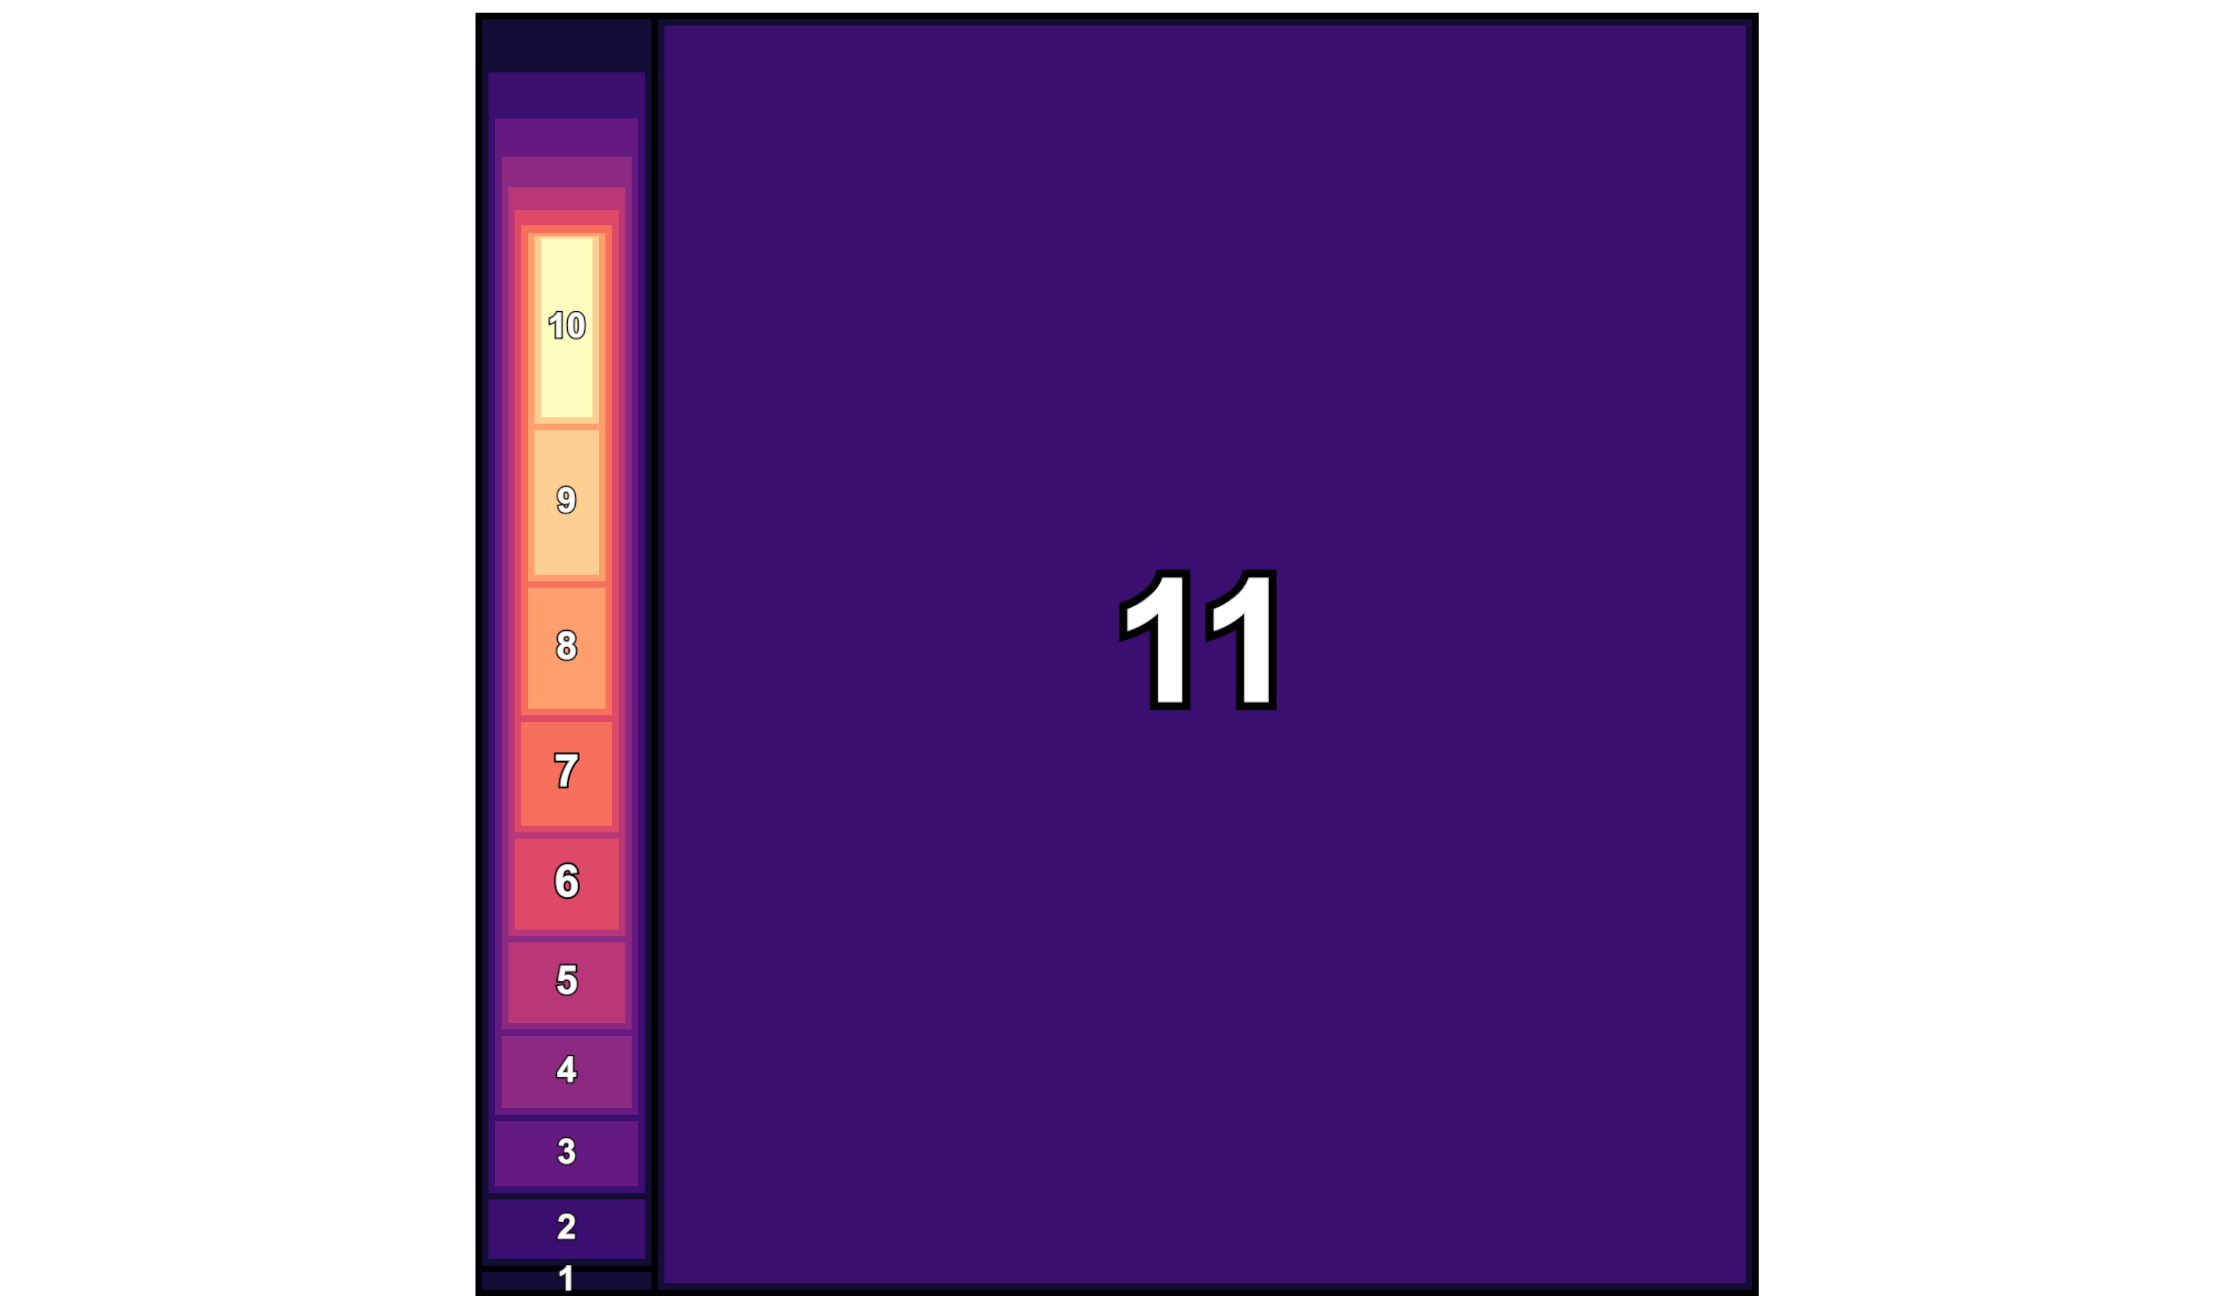
\includegraphics[width=0.8\textwidth]{images/increaseMarginOne.png}
    \caption{Treemap Layout generiert mit dem Squarify Algorithmus nach Abschnitt \ref{sec:Squarify} mit einem Abstand von 1 und der relativen Größenanpassung auf der händisch erstellen map (siehe Anhang).}
    \label{fig:relativeIncreaseMarginOne}
\end{figure}

\subsection{Scaling der Knoten} \label{sec:ScalingKnoten}
Wenn die Fläche innnerhalb von Elternknoten immer kleiner wird, kann es passieren, dass Knoten über ihre Elternknoten hinauswachsen, wie in Abbildung \ref{fig:simpleIncreaseMarginOne} zu sehen ist. Es kann genauso passieren, dass die Fläche innerhalb der Knoten größer wird, wie in Abbildung \ref{fig:relativeIncreaseMarginOne} auf der linken seite zu erkennen ist. Dieser Effekt kann trivialer weise behoben werden, indem der zweite Layout-Schritt angepasst wird, sodass die Knoten immer auf die Fläche des Elternknotens skaliert werden. 
Vor jeden Squarify-Schritt wird dafür die wirklich zur verfügung stehende Fläche des Elternknotens berechnet und die Kindknoten entsprechend dieser Änderung skaliert, sodass sie genau in die Fläche des Elternknotens passen.

Der Nachteil dieser Methode ist in Abbildung \ref{fig:simpleIncreaseMarginOneScale} zu erkennen. Die Knoten werden dadurch natürlich nicht mehr proportional zu ihren Werten sein. Knoten 10 hat zum beispiel ein Verhältnis von ca. 0.5 zu seinem Wert, während Knoten 6 ein Verhältnis von ca. 1.4 zu seinem Wert hat.

\begin{figure}
    \centering
    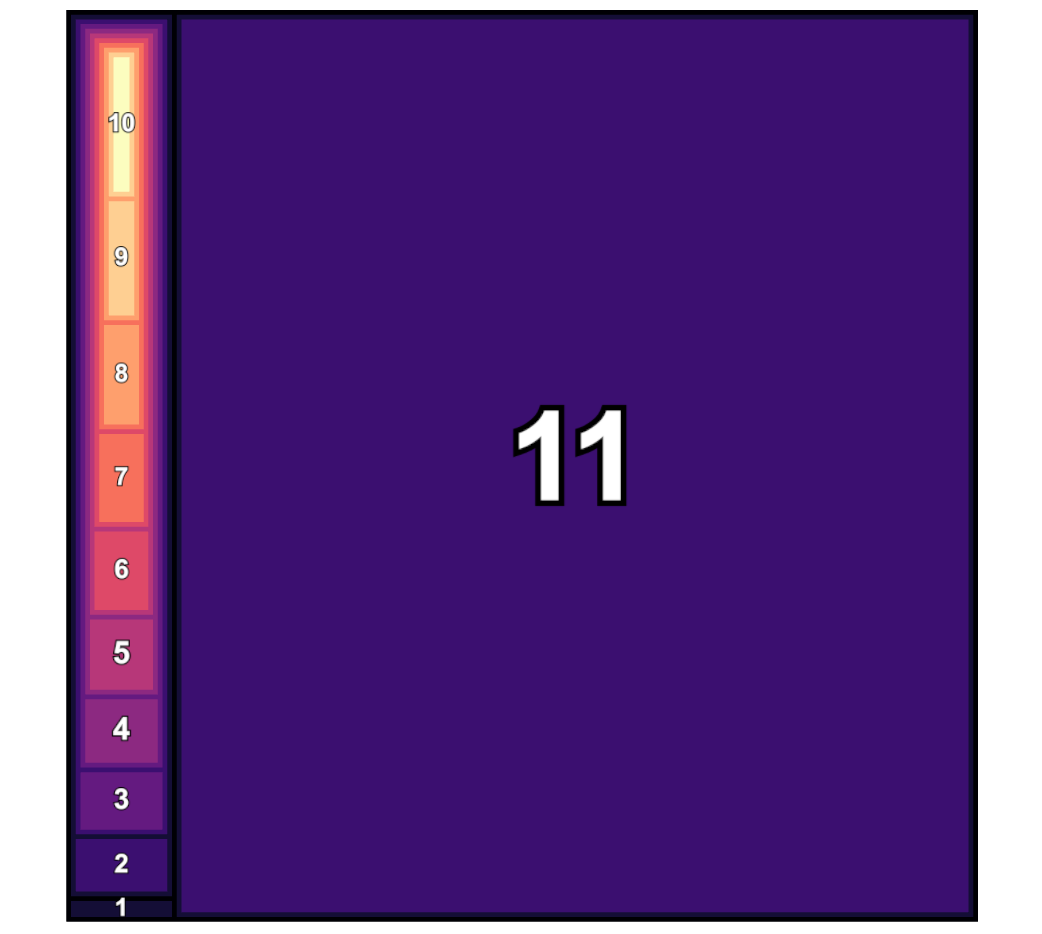
\includegraphics[width=0.8\textwidth]{images/simpleIncreaseMarginOneScale.png}
    \caption{Treemap Layout generiert mit dem Squarify Algorithmus nach Abschnitt \ref{sec:Squarify} mit einem Abstand von 1 und der einfachen Größenanpassung auf der händisch erstellen map (siehe Anhang) und der Skalierung der Knoten.}
    \label{fig:simpleIncreaseMarginOneScale}
\end{figure}

Je genauer die Größenanpassung der Knoten ist, desto geringer fällt natürlich dieser Effekt aus. Siehe im Vergleich dazu Abbildung \ref{fig:relativeIncreaseMarginOneScale}, da die relative Größenanpassung deutlich genauer ist, ist der Effekt hier auch deutlich geringer. Knoten 10 hat Größe 40 und Knoten 6 hat Größe 41, was fast ähnlich Groß ist.

\begin{figure}
    \centering
    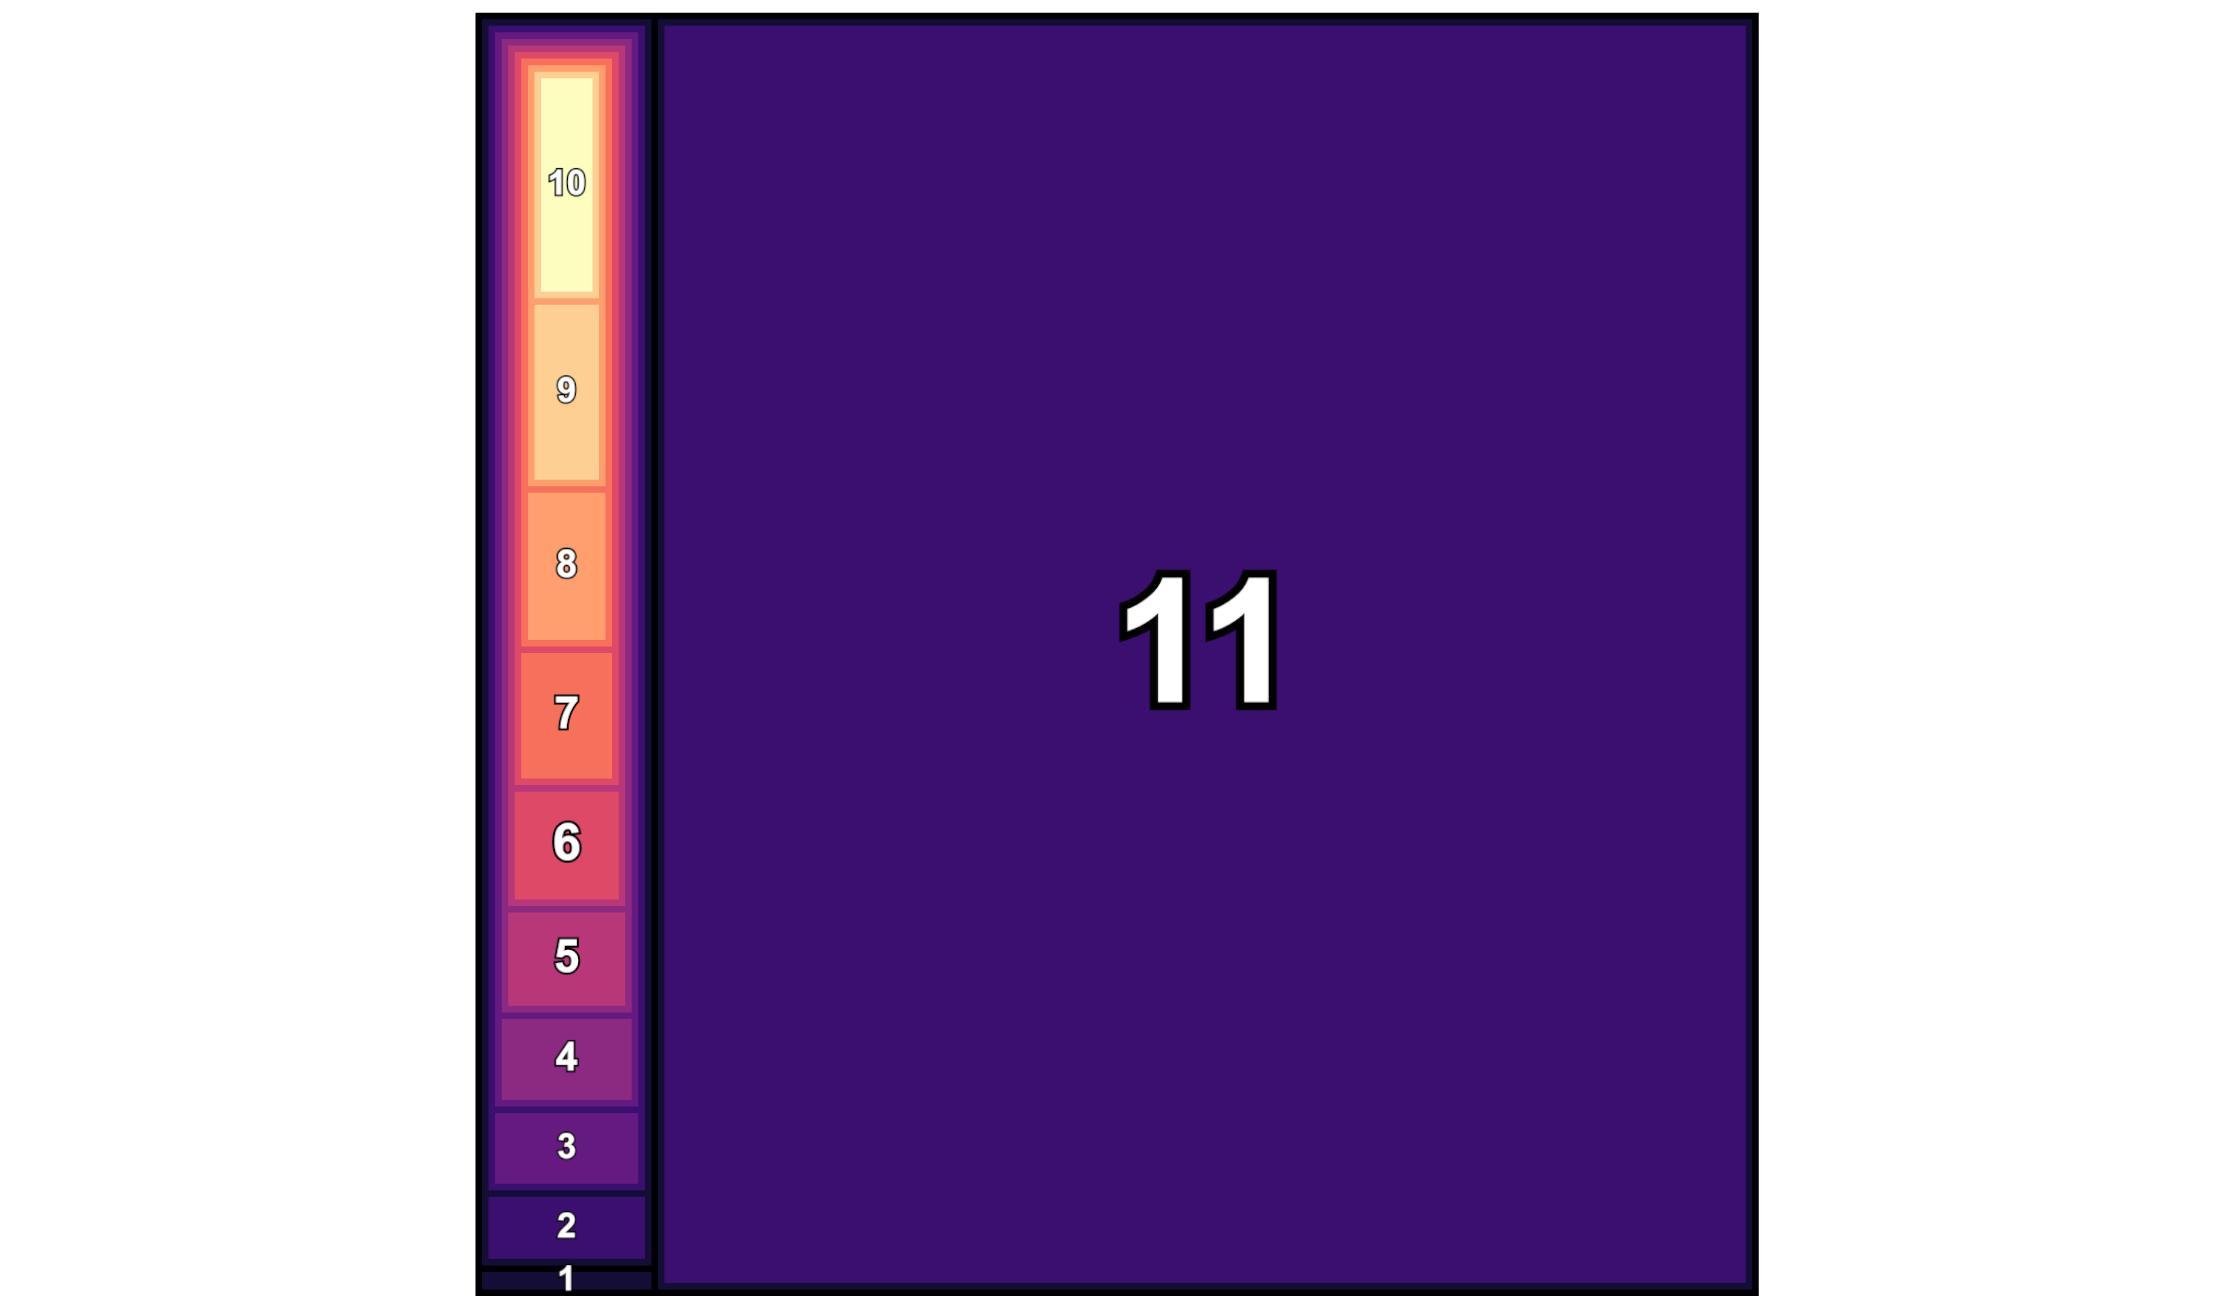
\includegraphics[width=0.8\textwidth]{images/increaseMarginOneScale.png}
    \caption{Treemap Layout generiert mit dem Squarify Algorithmus nach Abschnitt \ref{sec:Squarify} mit einem Abstand von 1 und der relativen Größenanpassung auf der händisch erstellen map (siehe Anhang) und der Skalierung der Knoten.}
    \label{fig:relativeIncreaseMarginOneScale}
\end{figure}

Persönlich würde ich sagen, dass dieser Effekt für das herunter skalieren der Knoten gut ist, da sonst eine grundlegende eigenschaft der Darstellung verletzt wird, aber für das hoch skalieren der Knoten könnte man auch sagen, dass es wichtiger ist die Fläche der Knoten proportional zu ihren Werten zu halten, als die \textit{verschwendete} Fläche aufzufüllen. Diese jetzt hier sehr subjektive Einschätzung wird aber nochmal genauer beläuchtet in der evaluation und vergleich.

\subsection{Reihenfolge der Knoten} \label{sec:ReihenfolgeKnoten}
Die Reienfolge in der die knoten in das Layout eingefügt werden, hat einen großen Einfluss auf das Layout. \cite{johnson1991tree} haben in ihrem Paper herausgefunden, dass die ergebnisse am besten sind, wenn die Knoten in der Reihenfolge der Größe eingefügt werden. Also der Größte zuerst.

\subsection{Mehrfache Berechnung} \label{sec:MehrfacheBerechnung}
Die Grundlegende Idee dieser Erweiterung ist es, das Layout mehrfach zu berechnen und dabei die Fläche der Knoten immer weiter anzupassen. Dies wird so lange wiederholt, bis sich die Fläche der Knoten nicht mehr ändert oder eine maximale Anzahl an Iterationen erreicht ist.

\subsection{Anpassung der Knoten}
In bild updateValues.png ist zu erkennen, dass kp. margin 10 noP 3


\subsection{Fazit}
Immernoch straight forward, es gibt aber noch Probleme 

Warum besonders den squarify algorithmus betrachtet und nicht zum beipsiel pivot oder circle?? -> weil diese Andere Ziele haben -> noch mehr begründen anhand der definierten Ziele


%weitere idee wie bei casced nach jedem layoutschritt im zweiten durchgang den benötigten platz neu berechnen



%schreibe warum die berechnung mit shrinkyfiy und nicht direct mit den margins plazieren
%ist mein shrinkify gleich zu setzen mit leafs nicht ändern und direkt mit margin platzieren?
%wenn alles genauso wie berechnet, dann egal, weil ich füge genauso viel platz hinzu, wie ich dann bei shrinkify abziehe
%wenn nicht alles genauso, dann für ich evtl. weniger platz hinzu als ich danach abziehe, weil sich die form der node ändert
%macht es am ende dann einen unterschied? weil ich würde dann die node ja trozdem scalen

%das scalen wird auch viel schwerer - weil, ja am anfang dann gar nicht klar ist wie viel platz benötigt wird für die abstände -> wäre das überhaupt möglich? 
%nein wäre es nicht, es müsste dann jede Row für sich gescaled werden -> interessanter ansatz, aber 


%Ideen: im shrink step, auf original größe shrinken -> wenn die zu größ ist, dann zumindest so dass margin hält
%Idee: einen dritten allgemeinen schritt für die siblingmargins einführen
%Idee: für sehr kleine nodes heuristisch, absolute werte hinzufügen -> oder dafür auch einen dritten schritt einfüren



%erkläre, warum wir immer ein seitenverhältnis von 1 anstreben. -> weil dadurch sogar näher am goldenen schnitt als mit phi, dadurch, dass nicht optimial, wird man immer "schlechter" sein, als der angestrebte ratio. vllt sogar grafisch zeigen, dass mit 1 besser ist. In d3.js zum beispiel wird phi verwendet, wir als autoren halte das für eine schlechte idee, aus den genannten gründen

\chapter{Schluss} \label{chapter:Schluss}
\section{evaluation} \label{sec:Evaluation}

Evaluation anhand eines echten beispiels mit verschiedenen Layouts.
In diesem Abschnitt werden 1. die verschiedenen Treemap-Algorithmen verglichen und anhand von konkreten Kriterien evaluiert, um den besten Algorithmus für die Visualisierung von Codequalitätsmetriken zu finden. 2. Werden alle vorgestellten Layouts anhand eines konkreten Beispiels aus der Praxis evaluiert.
Dies wird gemacht, indem eine echte, bereits durchgeführte, Software-Analyse nochmal mit den verschiedenen Layouts visualiert wird. Dann wird verschiedenen unerfahrenen Personen diese verschiedenen Visualierungen gezeigt und gefragt, wie sie die Software-Qualität einschätzen würden. Wenn das möglichst nahe an die Experten Einschätzung kommt, so wie es in der Analyse durchgeführt wurde, dann ist das Layout gut geeignet. 

\section{Kriterien für Treemap Layouts} \label{sec:CodeCityLayouts}
Um disese fünf Aspekte zu erreichen, definieren wir sechs Kriterien für das 2D layout, die diese Aspekte messbar machen. Diese Kriterien sollen helfen, die Qualität der Visualisierung zu bewerten und zu vergleichen. Die Kriterien sind:

\begin{itemize}
    \item \textbf{Abstände:} Abstände zwischen den Knoten verbessern die Übersichtlichkeit und die visuelle Komplexität.
    \item \textbf{Platznutzung:} Es sollte so wenig Fläche wir möglich ohne Informationsgehalt bleiben. Als gegenbeispiel kann man die Order-Knoten sehen, wie sie in der CodeCity Arbeit beschrieben wurden, bei denen die Fläche der Knoten nicht proportional zur Anzahl der Zeilen im Code ist, wodurch die Fläche an sich keinen Informationsgehalt mehr hat und außerdem viel leere Fläche entsteht.
    \item \textbf{Knoten sichtbarkeit:} Es sollte keine Knoten geben, die aufgrund von Abständen oder anderen Gründen nicht sichtbar sind. Dieses Ziel spielt speziell auf das in abschnitt \ref{sec:Treemap} beschriebene Problem ab.
    \item \textbf{Zeitaufwand:} Die Generierung des Layouts sollte in einem angemessenen Zeitrahmen erfolgen, um eine schnelle Visualisierung zu ermöglichen. Dies verbessert die Skalierbarkeit und generelle Nutzbarkeit der Visualisierung.
    \item \textbf{Seitenverhältnis:} Um die visuelle Komplexität zu reduzieren und die Verständlichkeit zu erhöhen, sollte das Seitenverhältnis der Knoten möglichst nahe bei 1:1 liegen. Dies verbessert die Lesbarkeit der Knoten und macht es einfacher, die Informationen zu erfassen.
    \item \textbf{Flächengröße:} Um die Korrelation mit dem Code zu gewährleisten, sollte die Fläche der Knoten proportional zum Metrikwert sein. (Hier ist noch unklar, ob das nur für Blätter gilt oder für alle Knoten)
    \item \textbf{Stabilität:} Die Knoten sollten bei Änderungen die Position und Größe beibehalten, um eine stabile Visualisierung zu gewährleisten. 
\end{itemize}

In dieser Arbeit sollen space filling approaches anaylsiert werden und speziell darauf untersucht werden, wie sie sich eignenen für die definierten anforderungen. Wie gut wird was erfüllt? Wann sollte man was anwenden? Kann eine gute kombination aus verschiedenen Ansätzen gefunden werden?
Bisher wurden im Grundlagenteil vorallem die splitting algorhtmen vorgestellt, aber es gibt natürlich auch andere Ansätze, die verfolgt werden können, um Treemap Layouts zu generieren. Zum beispiel gibt es bin packing oder optimierungs algorithmen. In dieser Arbeit sollen auch diese Ansätze betrachtet werden, um zu sehen, ob sie für die Visualisierung von Codequalitätsmetriken in einer space filling layout approach geeignet sind.

Dies soll getestet werden auf basis von verschiedenen öffentlichen Repositories, die von kleinen bis großen Codebasen reichen. Als Metrik für die Fläche soll der Einfachehit halber die Anzahl der Zeilen verwendet werden.



%*************************************************************************
% Recommendations
%*************************************************************************
%\part{Empfehlungen zur Erstellung wissenschaftlicher Abschlussarbeiten}
%\label{pt:recommendations}
%*************************************************************************
% Backmatter
%*************************************************************************
\appendix
%\renewcommand{\thechapter}{\alph{chapter}}
\cleardoublepage
\part{Appendix}
%\include{chapters/examples/appendix01}
%\include{chapters/examples/appendix02}
%hier noch anhänge anhängen
anhang/artificial.cc.json

%*************************************************************************
% Other Stuff in the Back
%*************************************************************************
\cleardoublepage%********************************************************************
% Bibliography
%*******************************************************
% work-around to have small caps also here in the headline
% https://tex.stackexchange.com/questions/188126/wrong-header-in-bibliography-classicthesis
% Thanks to Enrico Gregorio
\defbibheading{bibintoc}[\bibname]{%
  \phantomsection
  \manualmark
  \markboth{\spacedlowsmallcaps{#1}}{\spacedlowsmallcaps{#1}}%
  \addtocontents{toc}{\protect\vspace{\beforebibskip}}%
  \addcontentsline{toc}{chapter}{\tocEntry{#1}}%
  \chapter*{#1}%
}

% allow Linebreaks in urls anywhere
\setcounter{biburlnumpenalty}{100}
\setcounter{biburlucpenalty}{100}
\setcounter{biburllcpenalty}{100}
% enable to long words to break anywhere by increasing the allowed whitespace between words.
\sloppy

\printbibliography[heading=bibintoc]

%*************************************************************************
% Game Over: Restore, Restart, or Quit?
%*************************************************************************
\end{document}
%*************************************************************************
